\section{Results}
In this section, we present the final results. Additionnally to these results,
we also provide tuning results that have guided our algorithm selection.

\subsection{F1}
Figure~\ref{fig:f1} shows the f1-scores for four datasets: \banosdataset,
RandomTree, \recofitdataset, and \banosdataset with a drift in the middle.  We
observe that on the long run, the Mondrian algorithm with 5 and 10 trees, and
the Naive Bayes algorithms present the best f1-scores. We also observe that the
NaiveBayes algorithms start faster than the Mondrian.

On Figure~\ref{fig:f1}, we can see two type of MCNN: MCNN Origin and MCNN
OrpailleCC. Both algorithm are implemented in the library OrpailleCC, however
MCNN Origin strictly follow the algorithm described in~\cite{mc-nn} where as
MCNN OrpailleCC tweak this algorithm to ensure a fixed memory footprint. The
difference appears on how micro-clusters are removed. MCNN-Origin removes a
micro-cluster when its participation falls below a threshold given by the user
"tandis que" MCNN-OrpailleCC remove the micro-cluster with the least
participation when the maximum number of micro-cluster is reached and we need
to introduce a new one.

Figure~\ref{fig:f1} shows that in all cases, MCNN-OrpailleCC achieves better
performance than its MCNN-Origin counter-part. Additionnally, most of the time,
any MCNN-OrpailleCC performs better than all MCNN-Origin.

Surprisingly, we note that using 50 trees with th Mondrian algorithm show worse
f1-scores than using 5 or 10. This unexpected results appears because the
Mondrian implementation forces a fixed memory footprint. Therefore, the tree
growth are blocked when there is not enought memory. Because 50 trees fill the
memory faster than 10 or 5 trees, the classifier adaptation is blocked faster,
when the trees have not learn enough from the data. However, when the memory
available is increased, using 50 trees achieve better f1-scores than using 10
trees.

Figure~\ref{fig:f1-drift} shows the F1-score when an artificial drift is
applied on the \banosdataset. We observe that the f1-score of the Mondrian
algorithm as well as the NaiveBayes suffer from the drift and they cannot adapt
to it. We also note that after a small set back, the HoeffdingTree algorithm
gets its f1-score to increase again. Finally, we barely notice any change on
the f1-score of the MCNNs. Only the highest MCNN (MCNN-OrpailleCC with 33, 40,
and 50 clusters) have a slight decrease.

Regarding the StreamDM HoeffdingTree algorithm, we can see that it matches very
closely the StreamDM NaiveBayes. This happens because the HoeffdingTree uses a
NaiveBayes in the leaves. However after a large number of element or after a
drift, we notice that two start diverging.

\begin{figure}[H]
	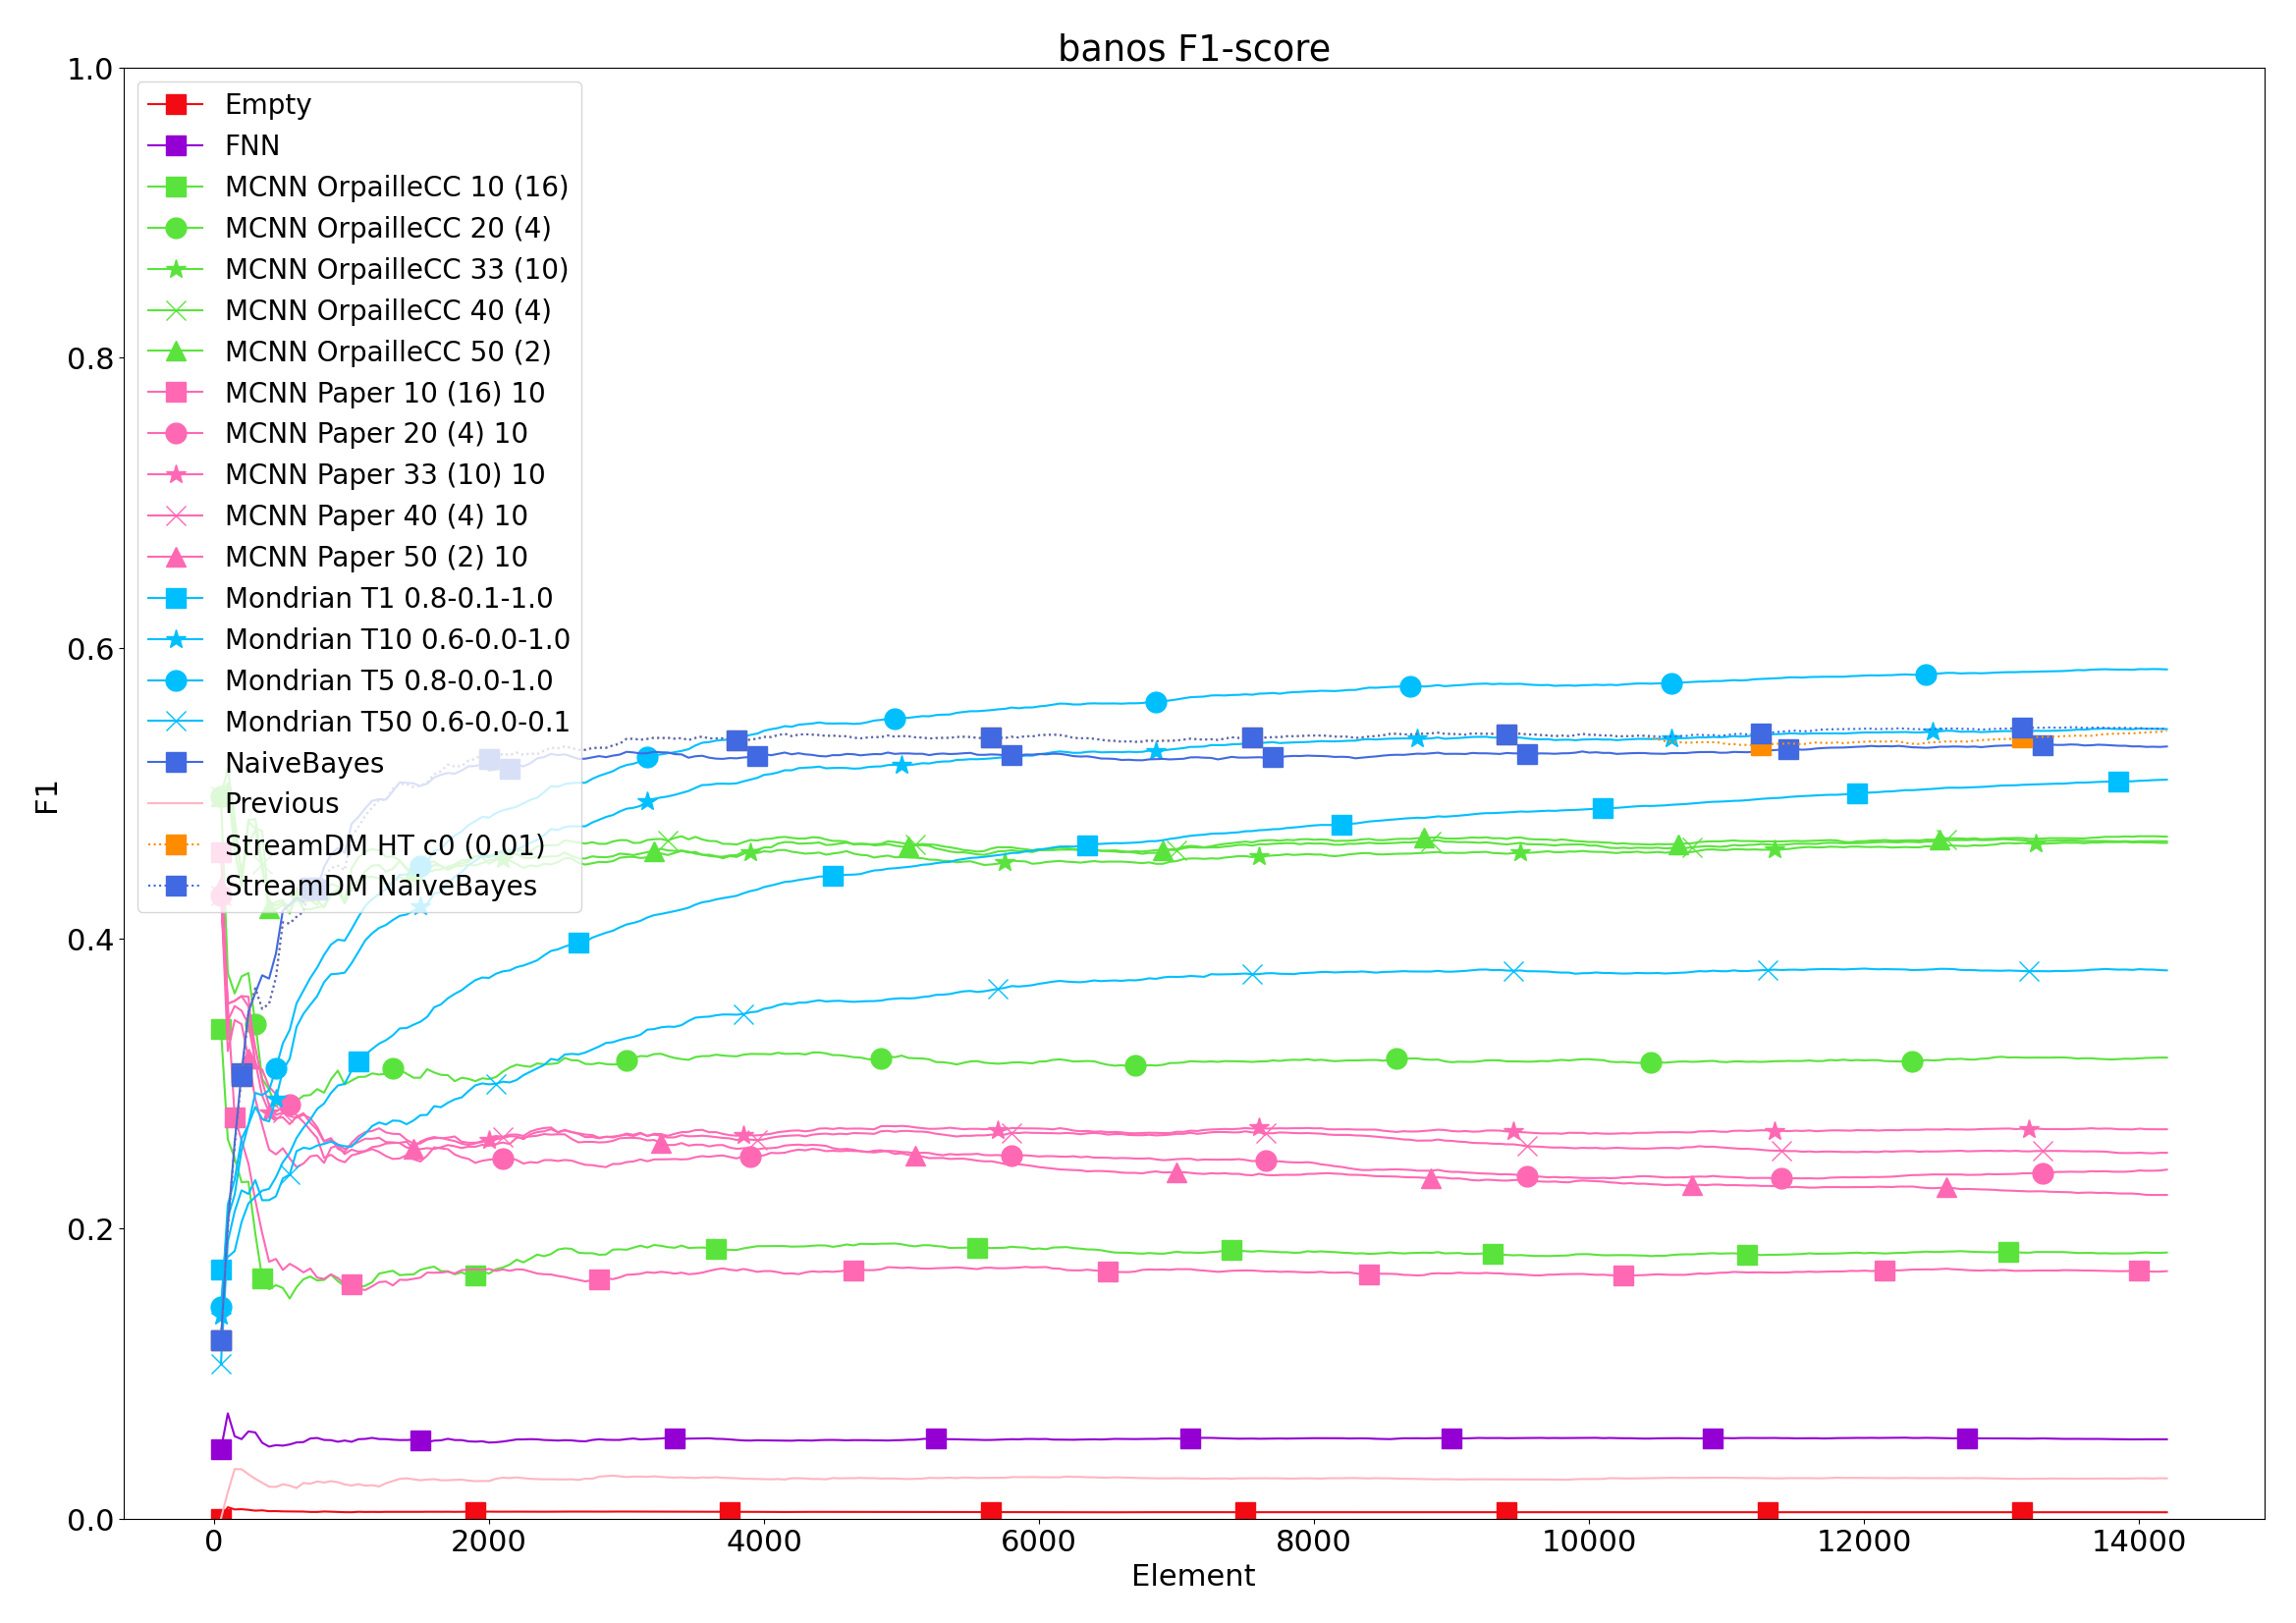
\includegraphics[width=\linewidth]{figures/results/banos_f1.png}
	\caption{F1-score on the Banos dataset.}
\end{figure}
\begin{figure}[H]
	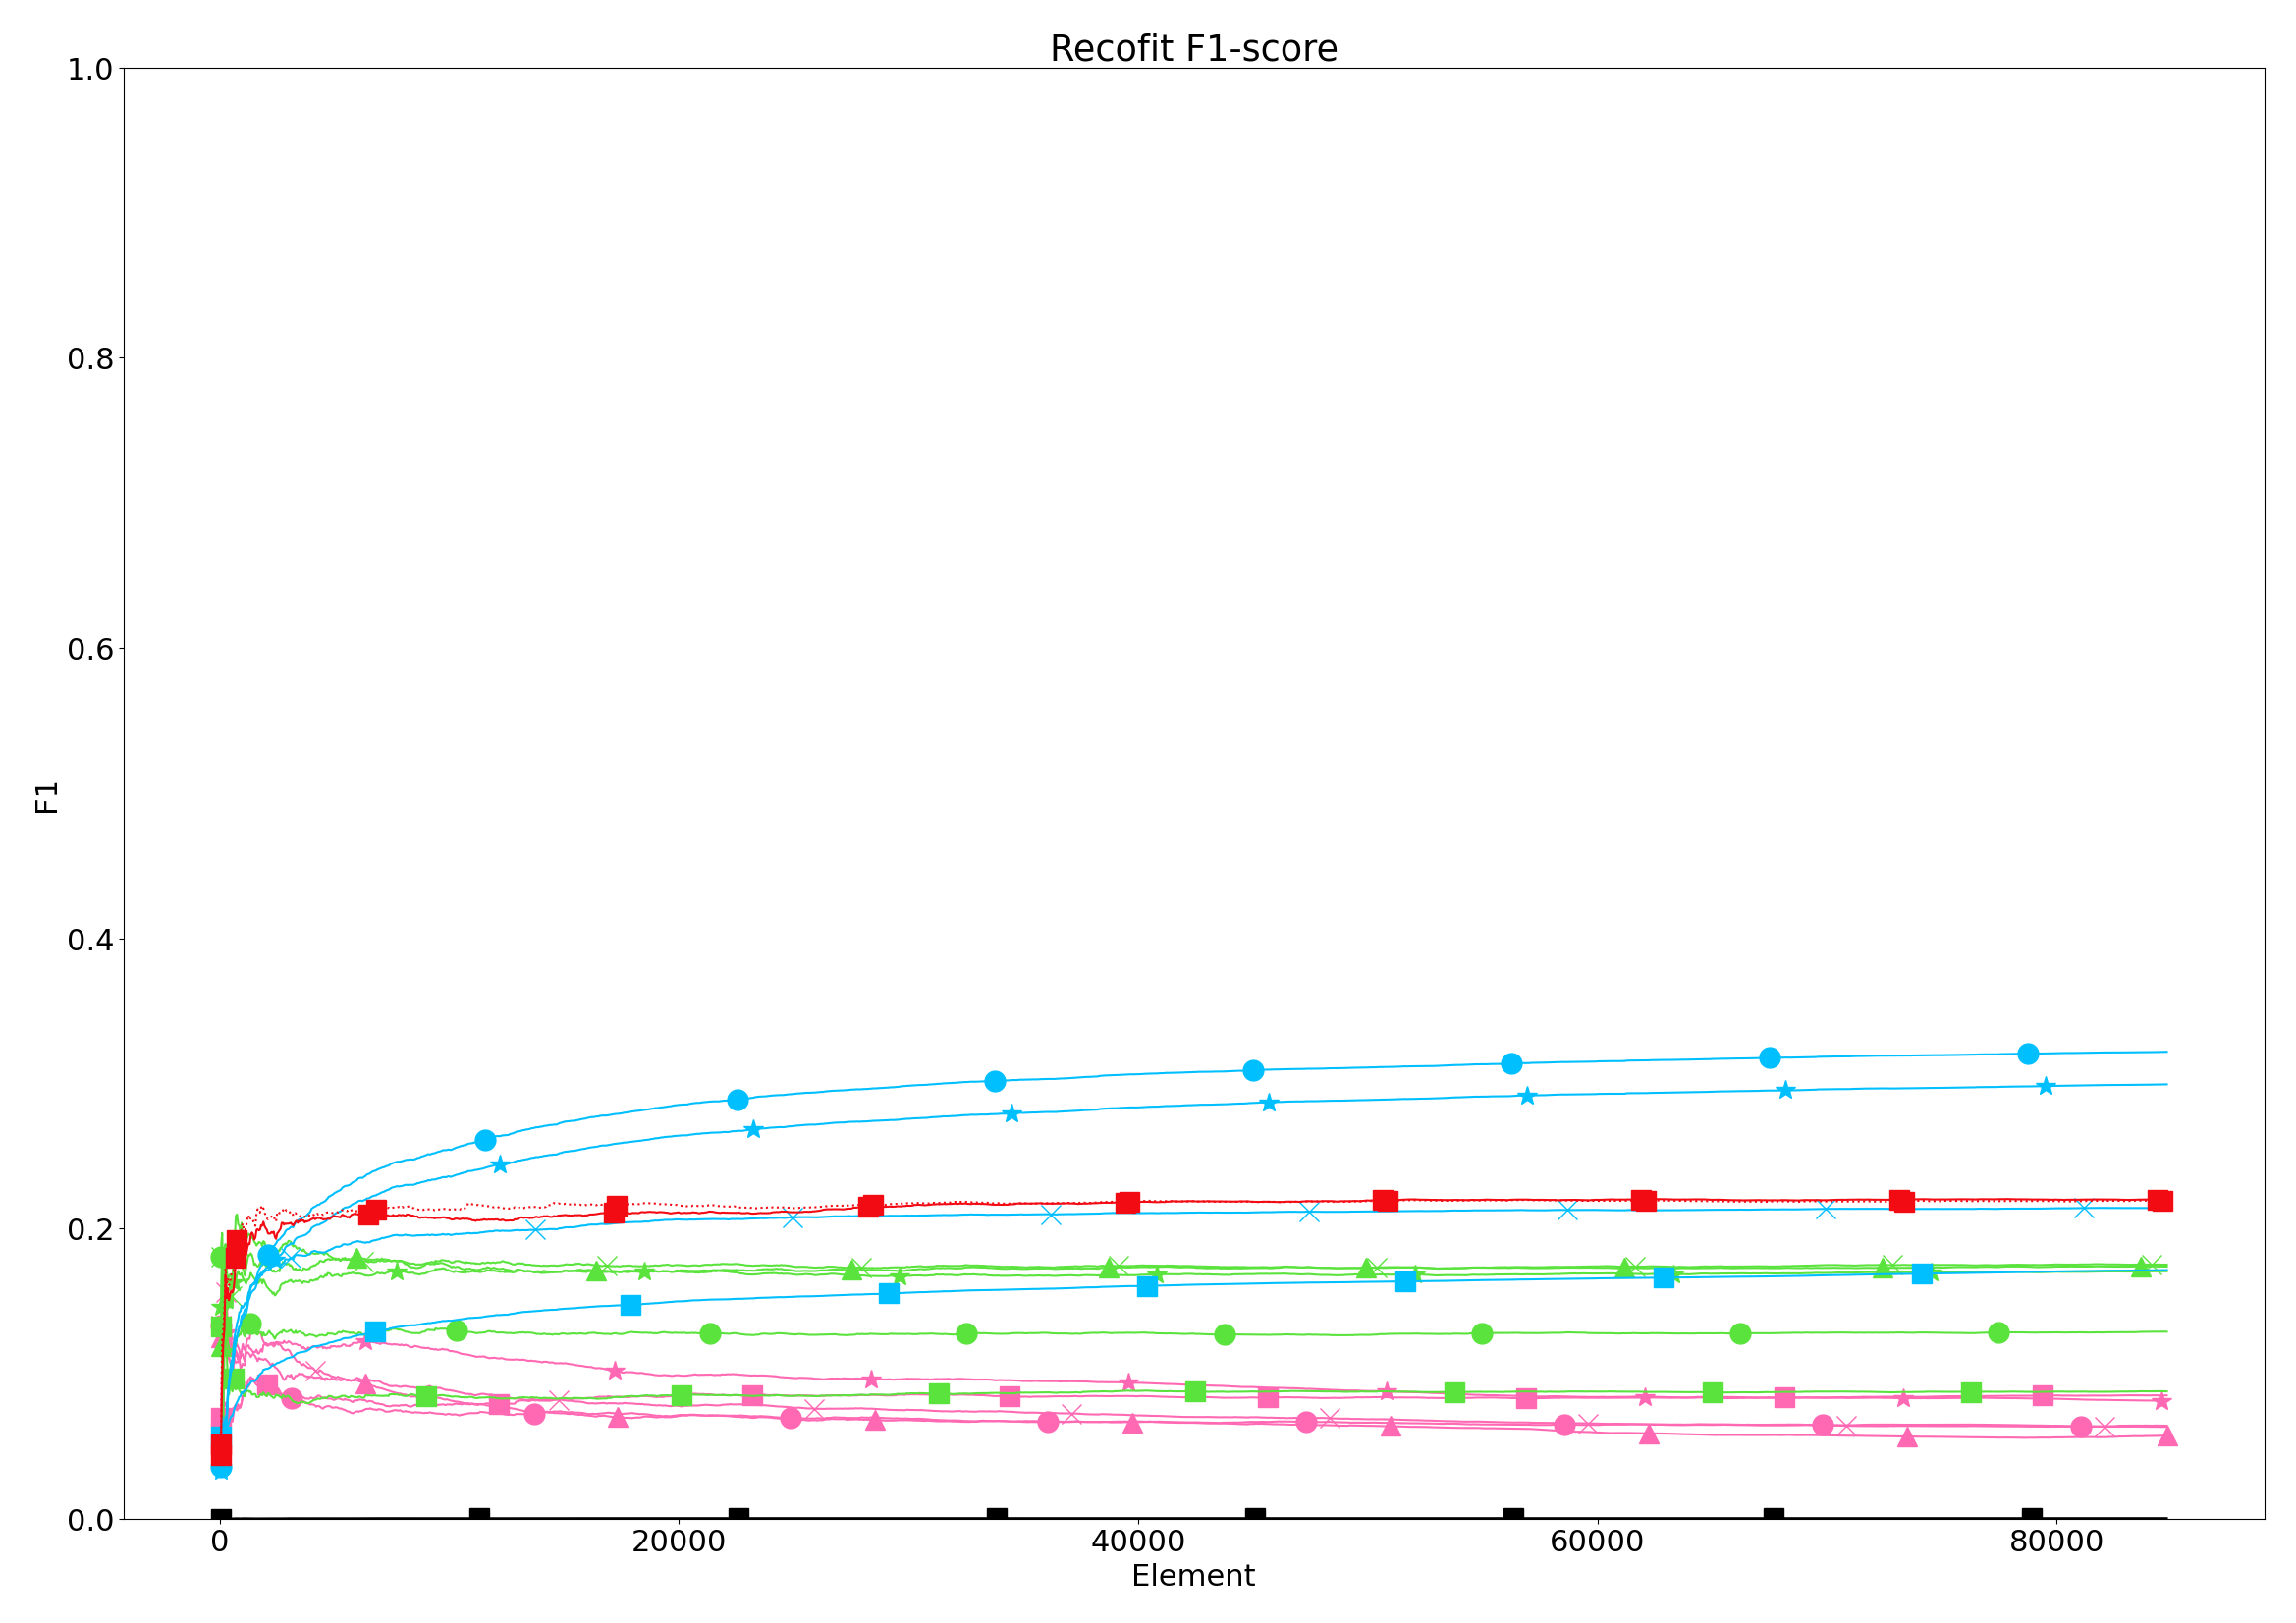
\includegraphics[width=\linewidth]{figures/results/recofit_f1.png}
	\caption{F1-score on the Recofit dataset.}
\end{figure}
\begin{figure}[H]
	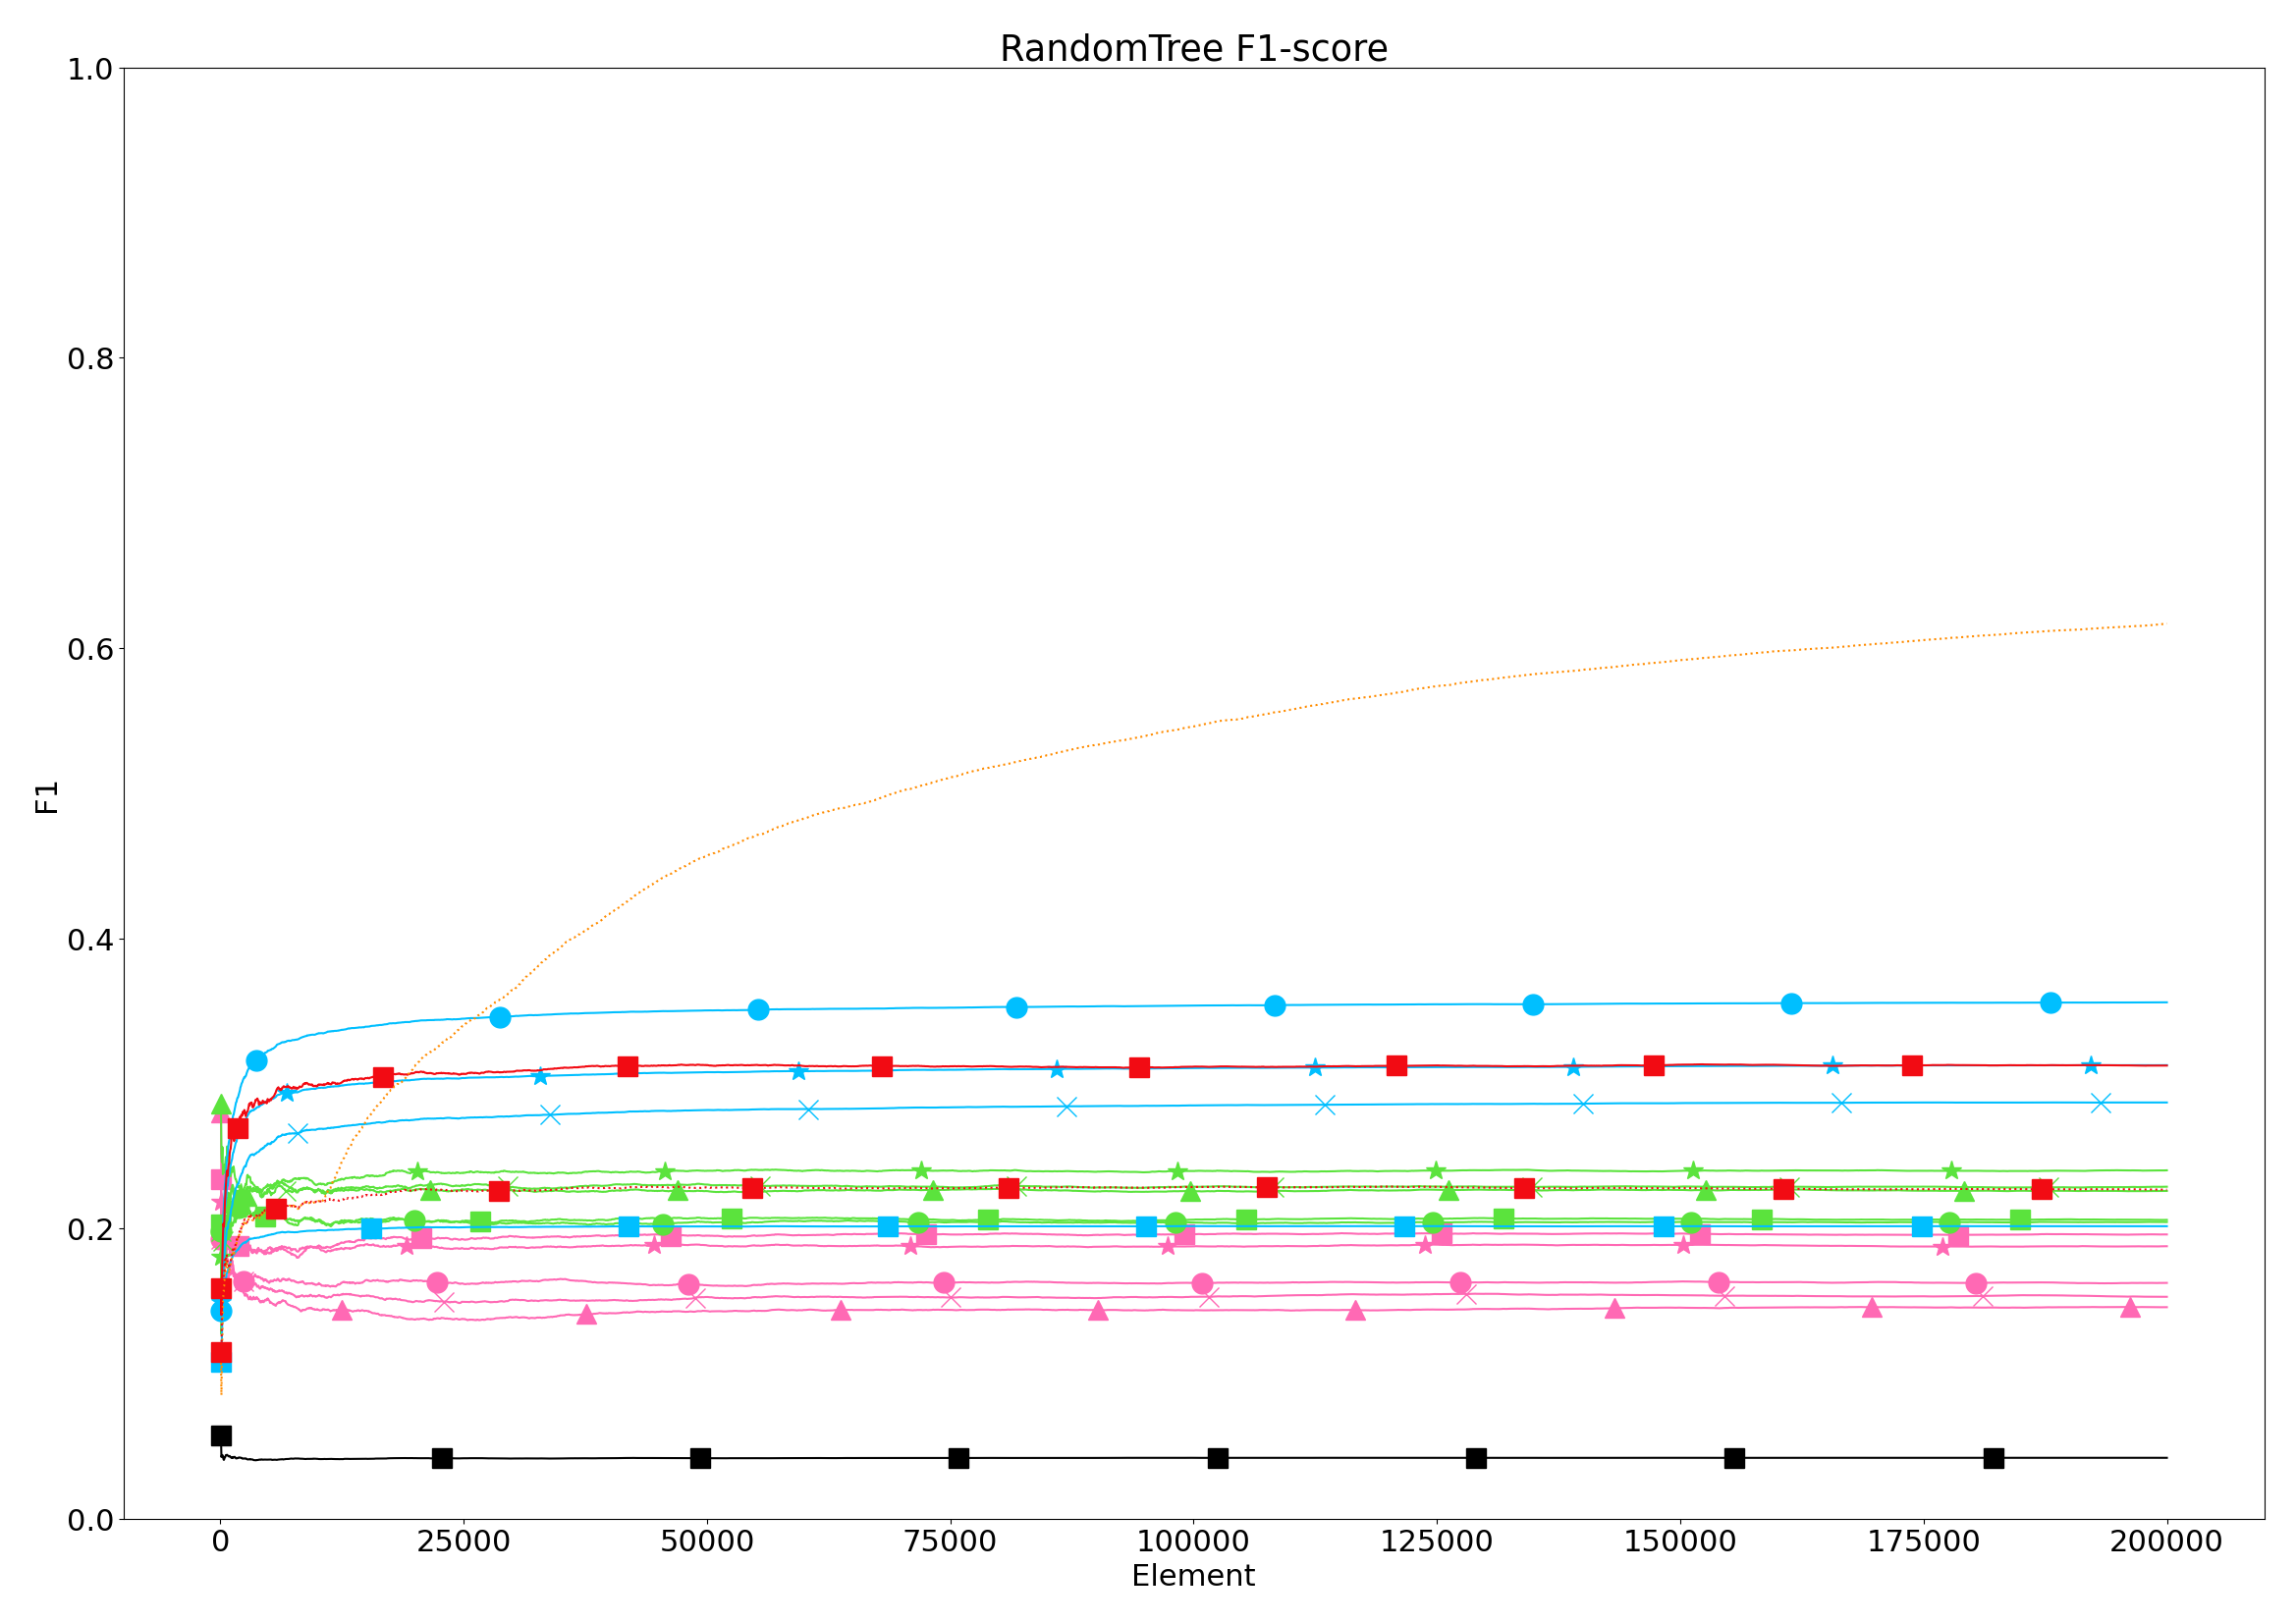
\includegraphics[width=\linewidth]{figures/results/dataset_3_f1.png}
	\caption{F1-score on the third synthetic dataset.}
\end{figure}
\begin{figure}[H]
	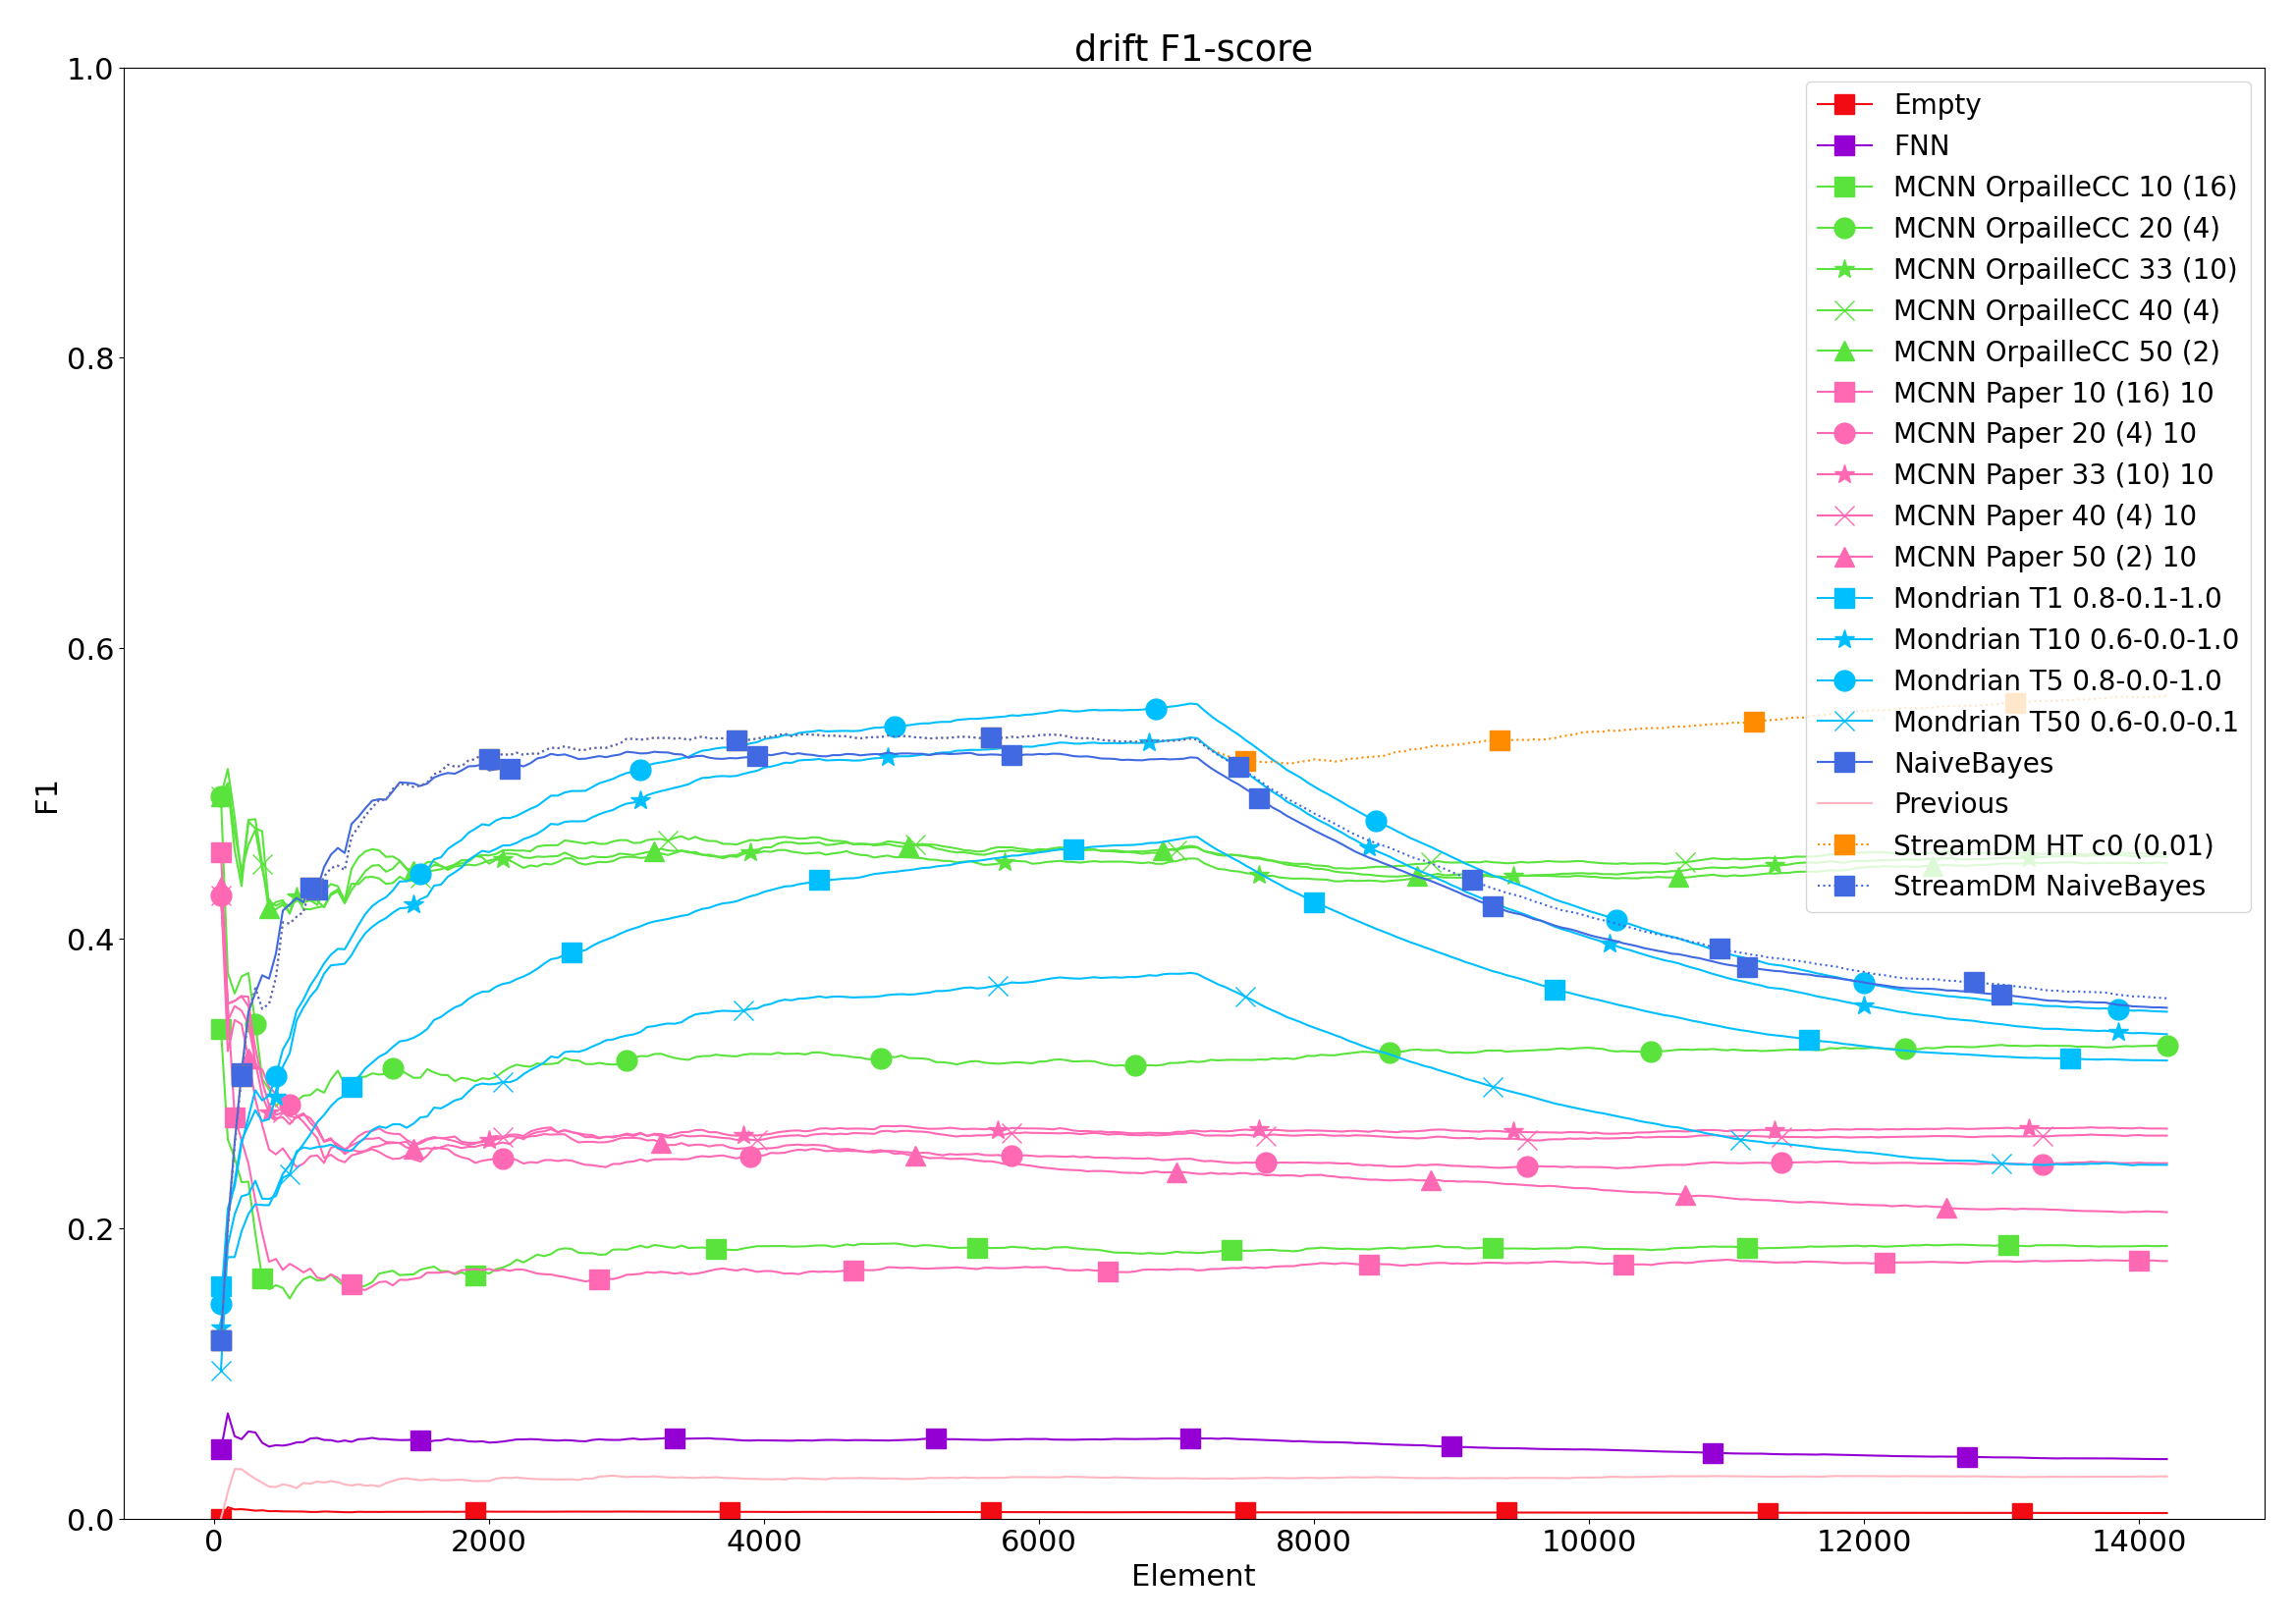
\includegraphics[width=\linewidth]{figures/results/drift_f1.png}
	\caption{Impact of an artificial drift.}
	\label{fig:f1-drift}
\end{figure}

\subsection{Power}
\begin{figure}[H]
	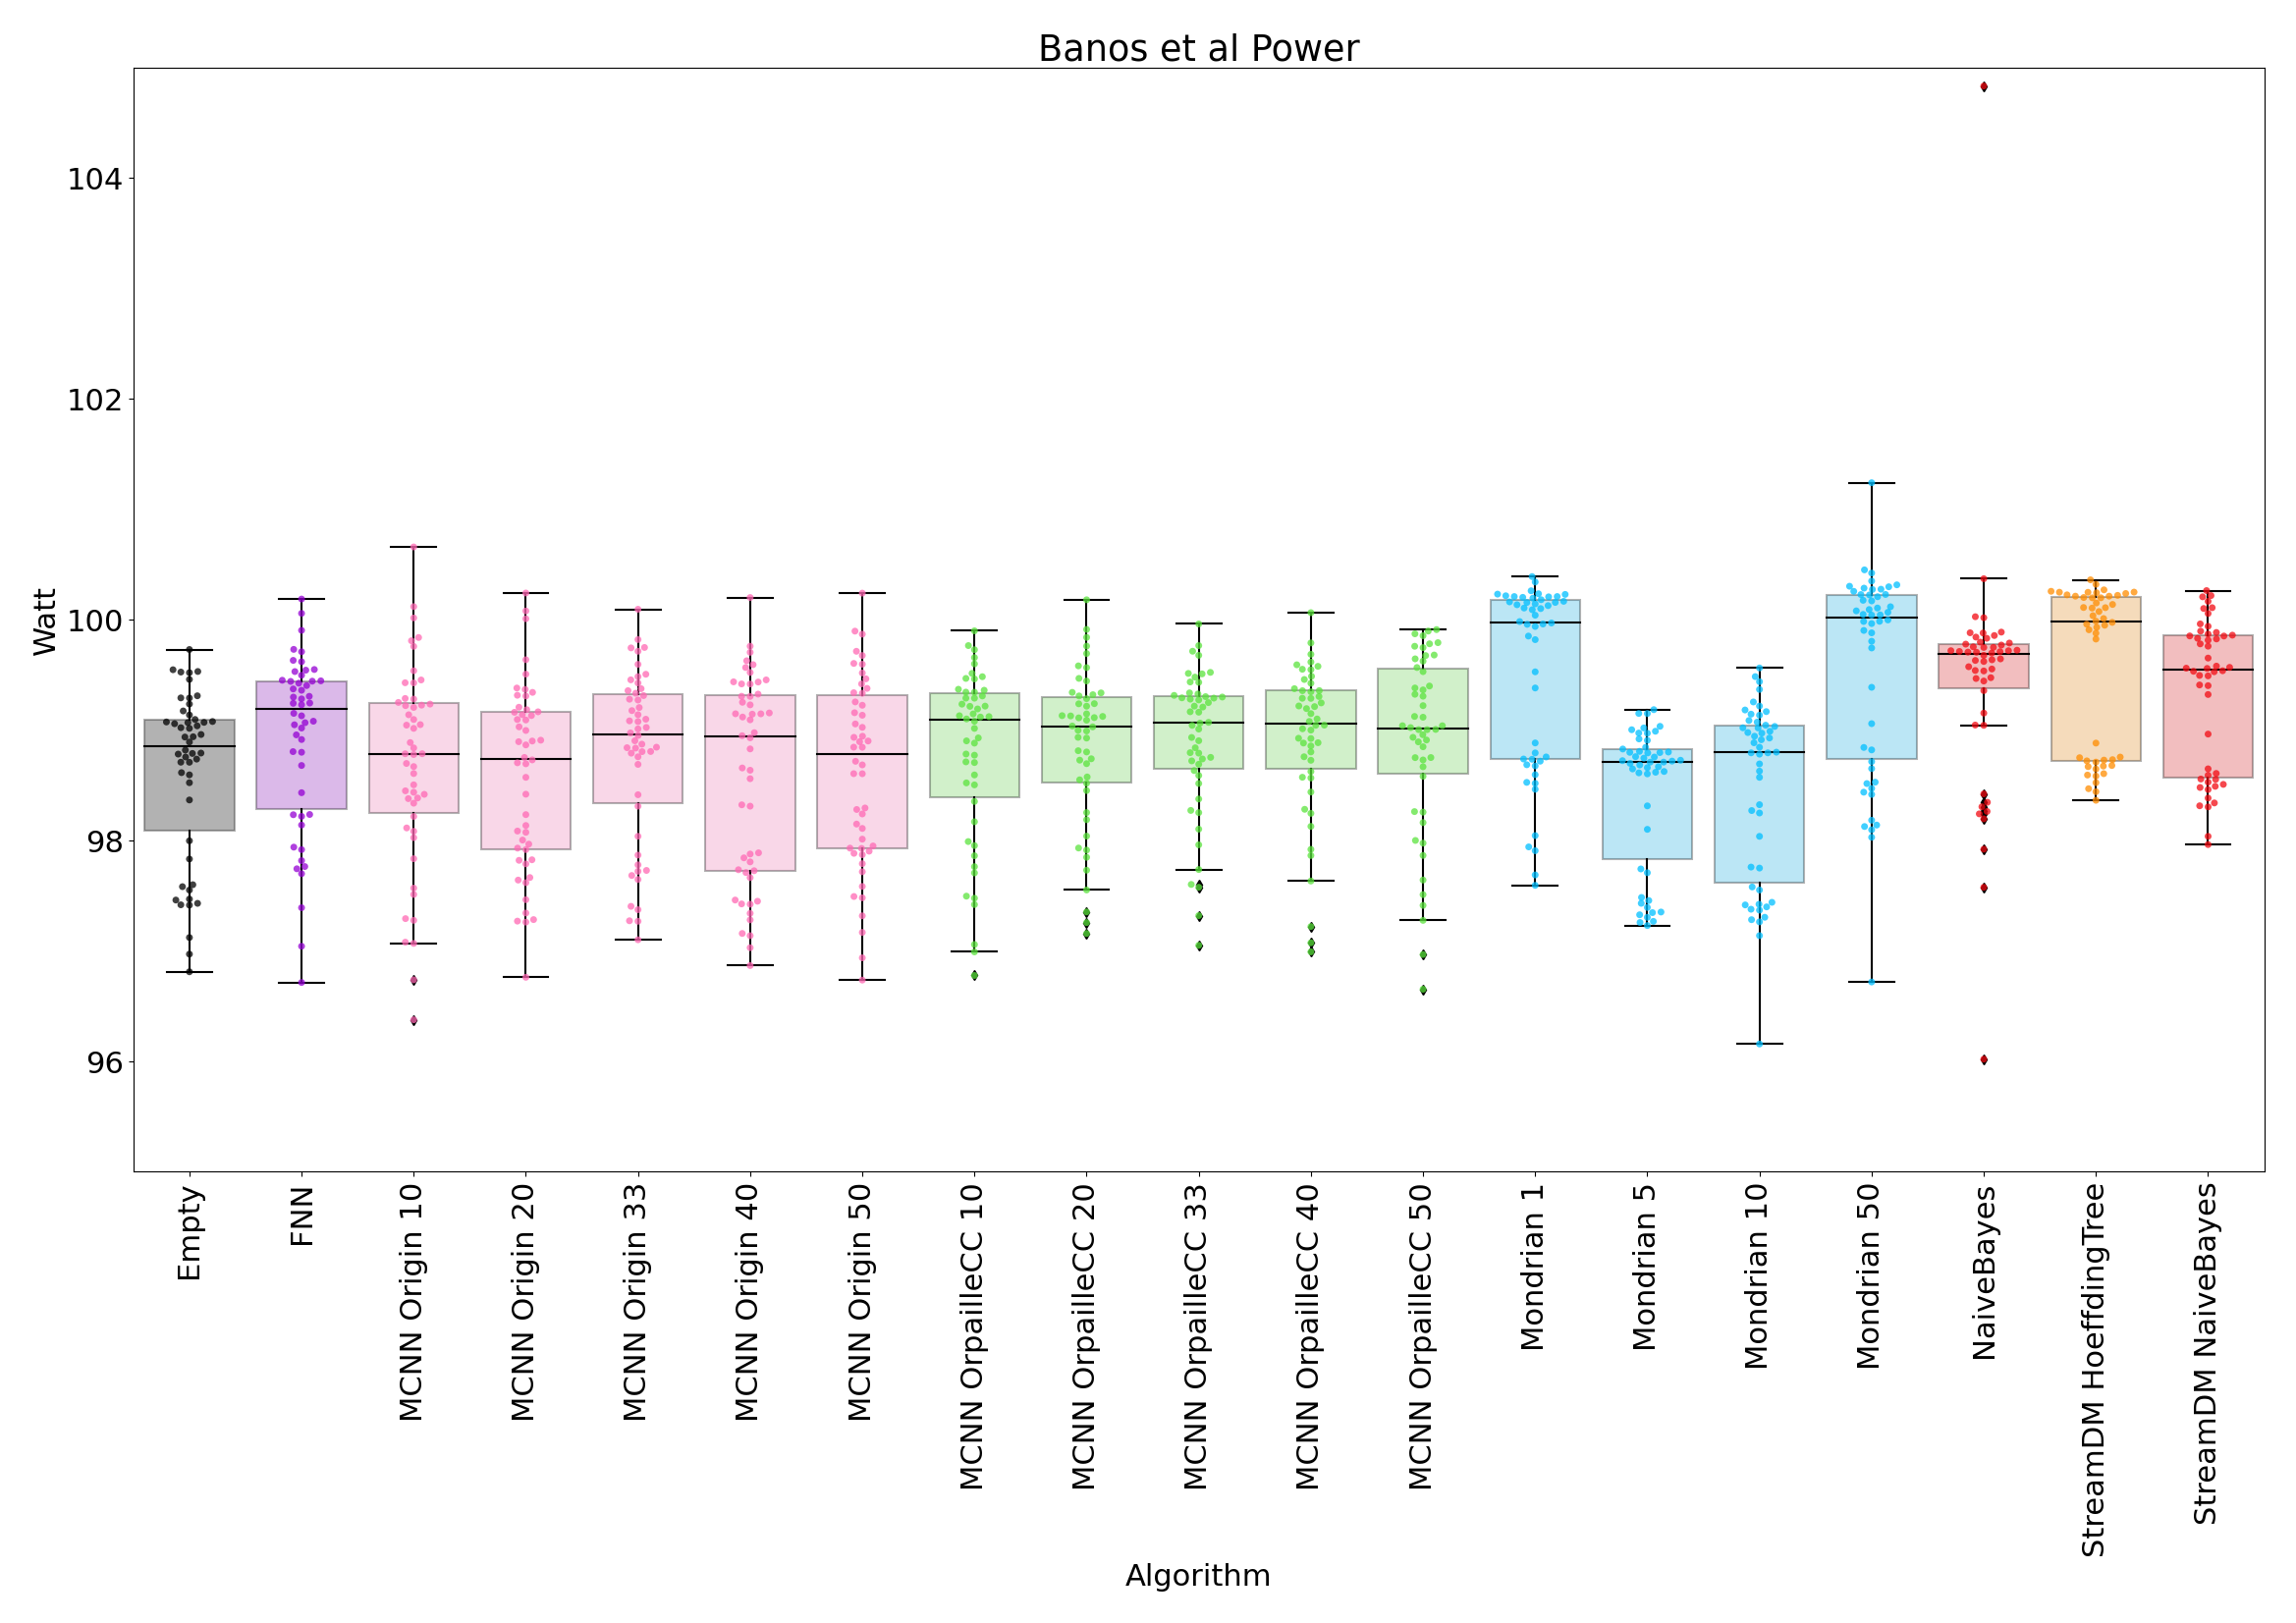
\includegraphics[width=\linewidth]{figures/results/banos_watt.png}
	\caption{Power needed for each algorithm on the Banos dataset.}
\end{figure}
\begin{figure}[H]
	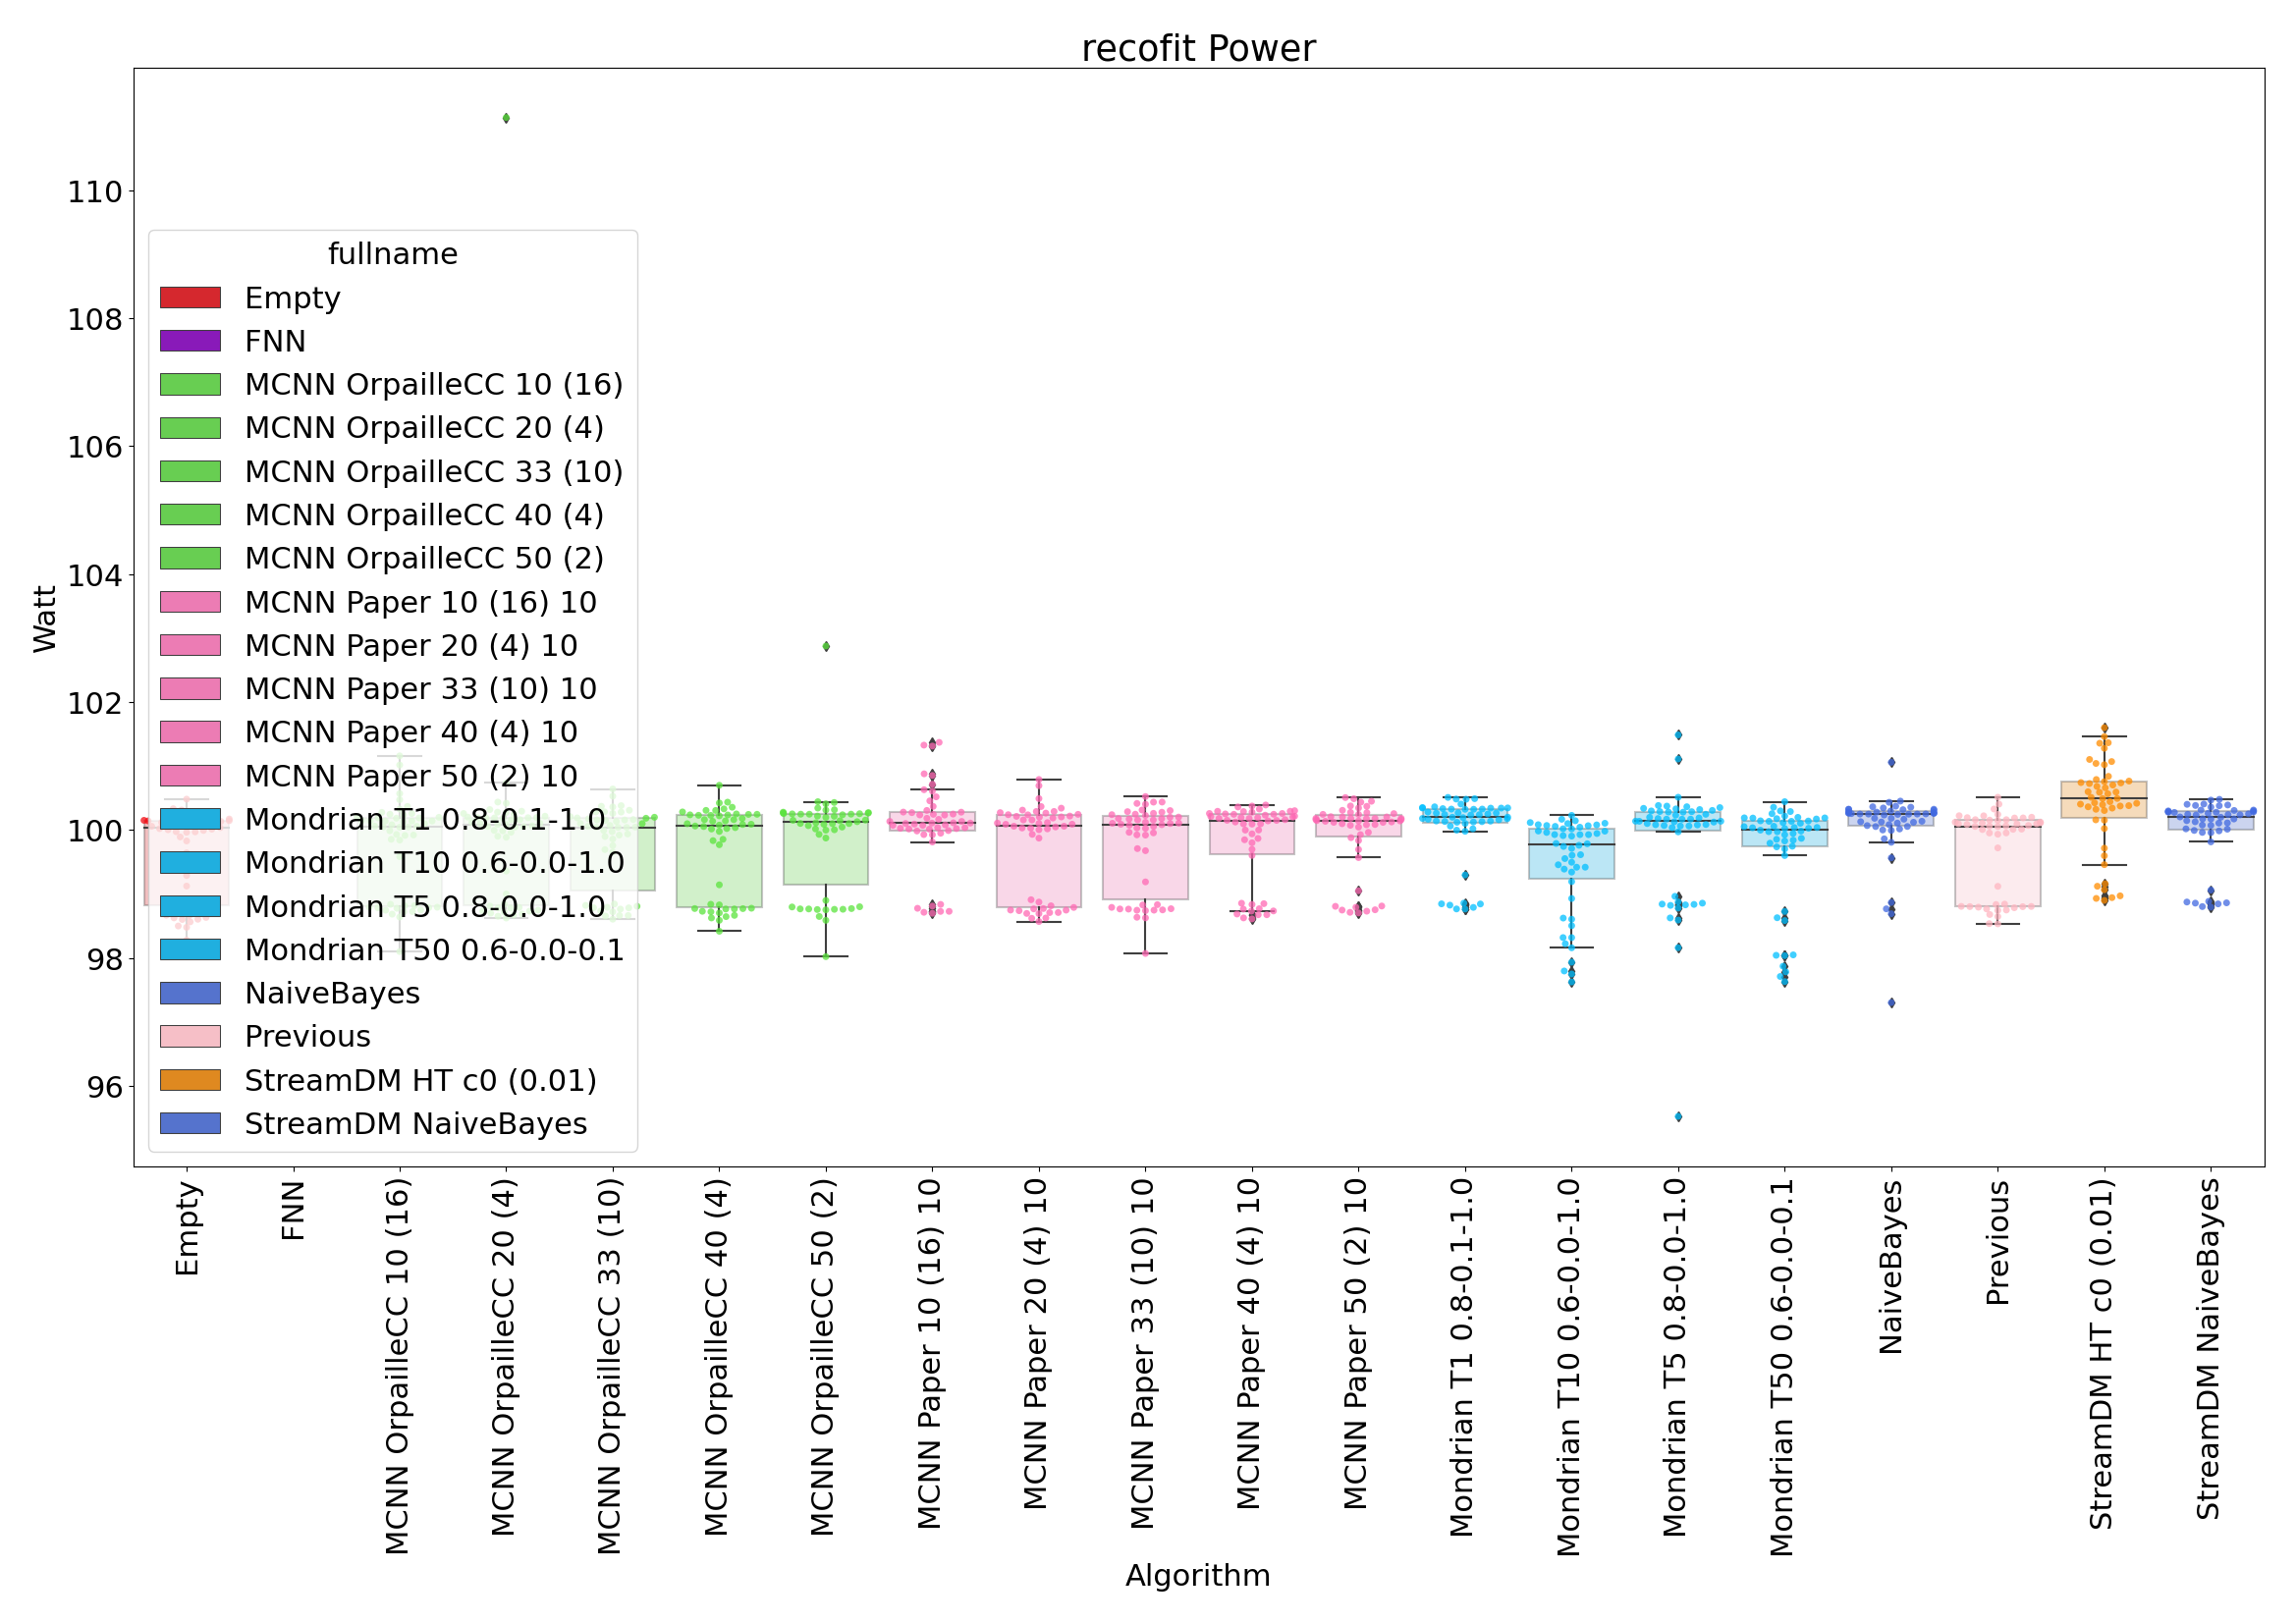
\includegraphics[width=\linewidth]{figures/results/recofit_watt.png}
	\caption{Power needed for each algorithm on the Recofit dataset.}
\end{figure}
\begin{figure}[H]
	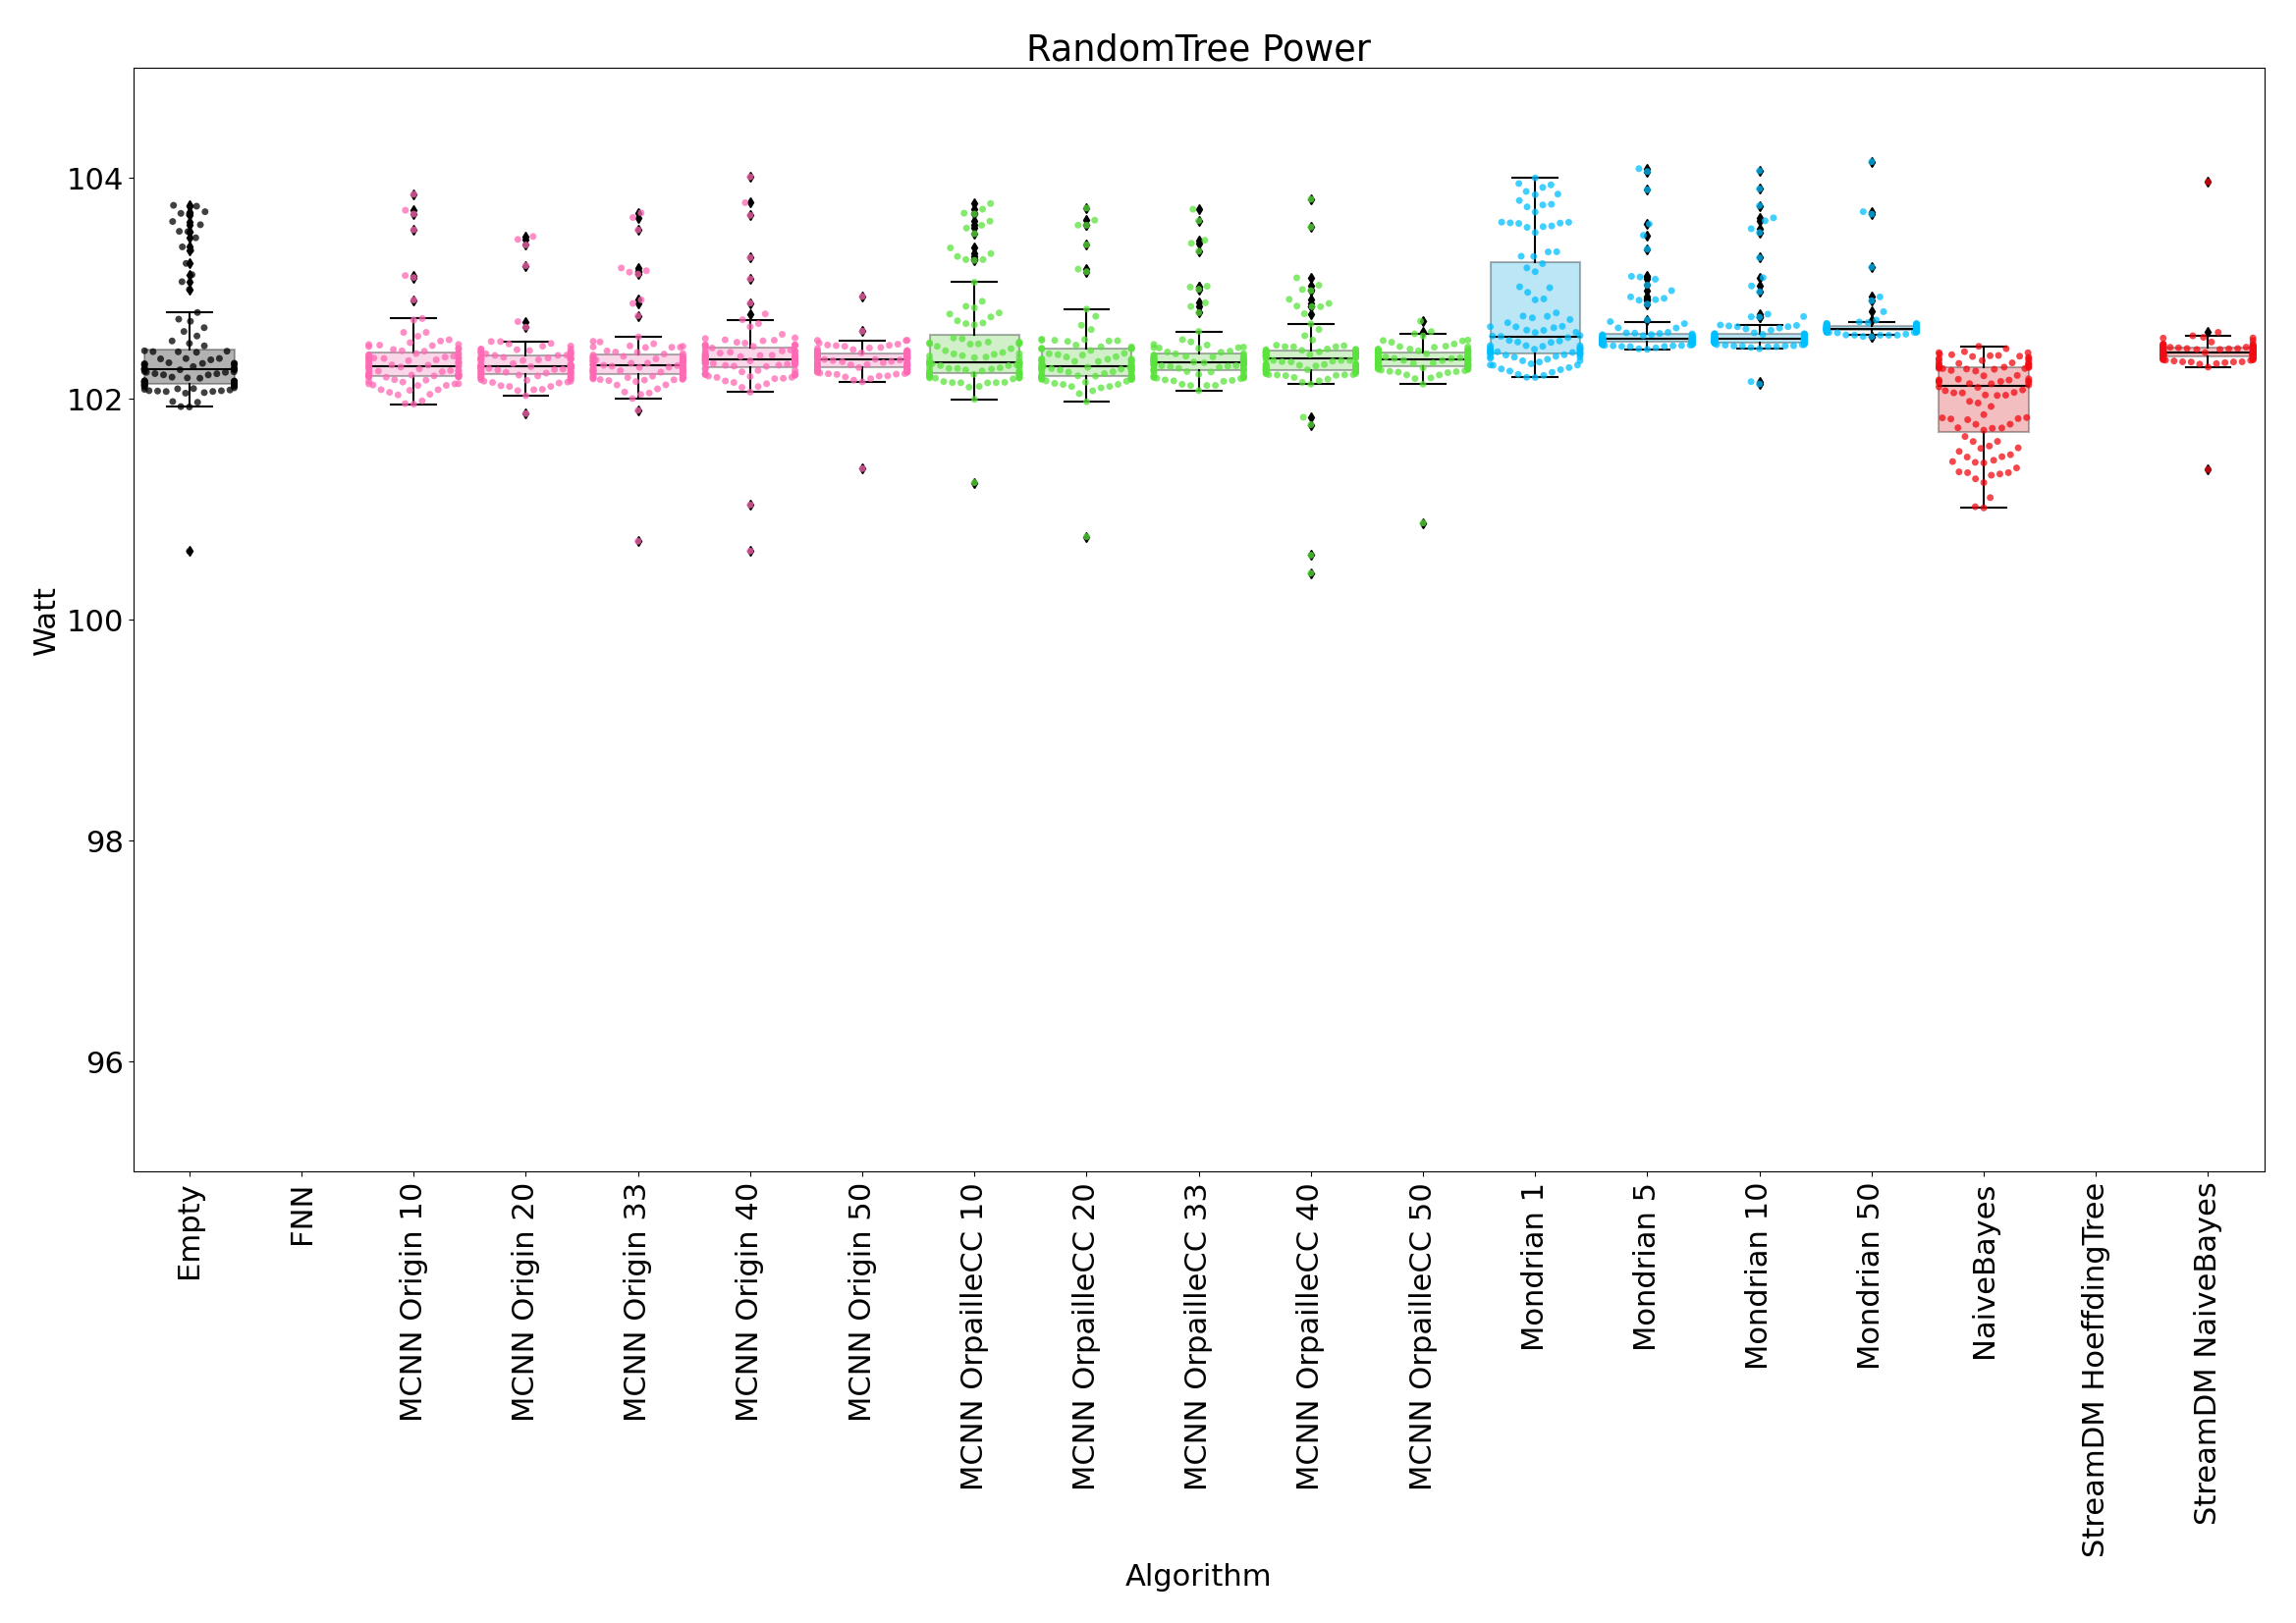
\includegraphics[width=\linewidth]{figures/results/dataset_3_watt.png}
	\caption{Power needed for each algorithm on the third synthetic dataset.}
\end{figure}

\subsection{Runtime}
\begin{figure}[H]
	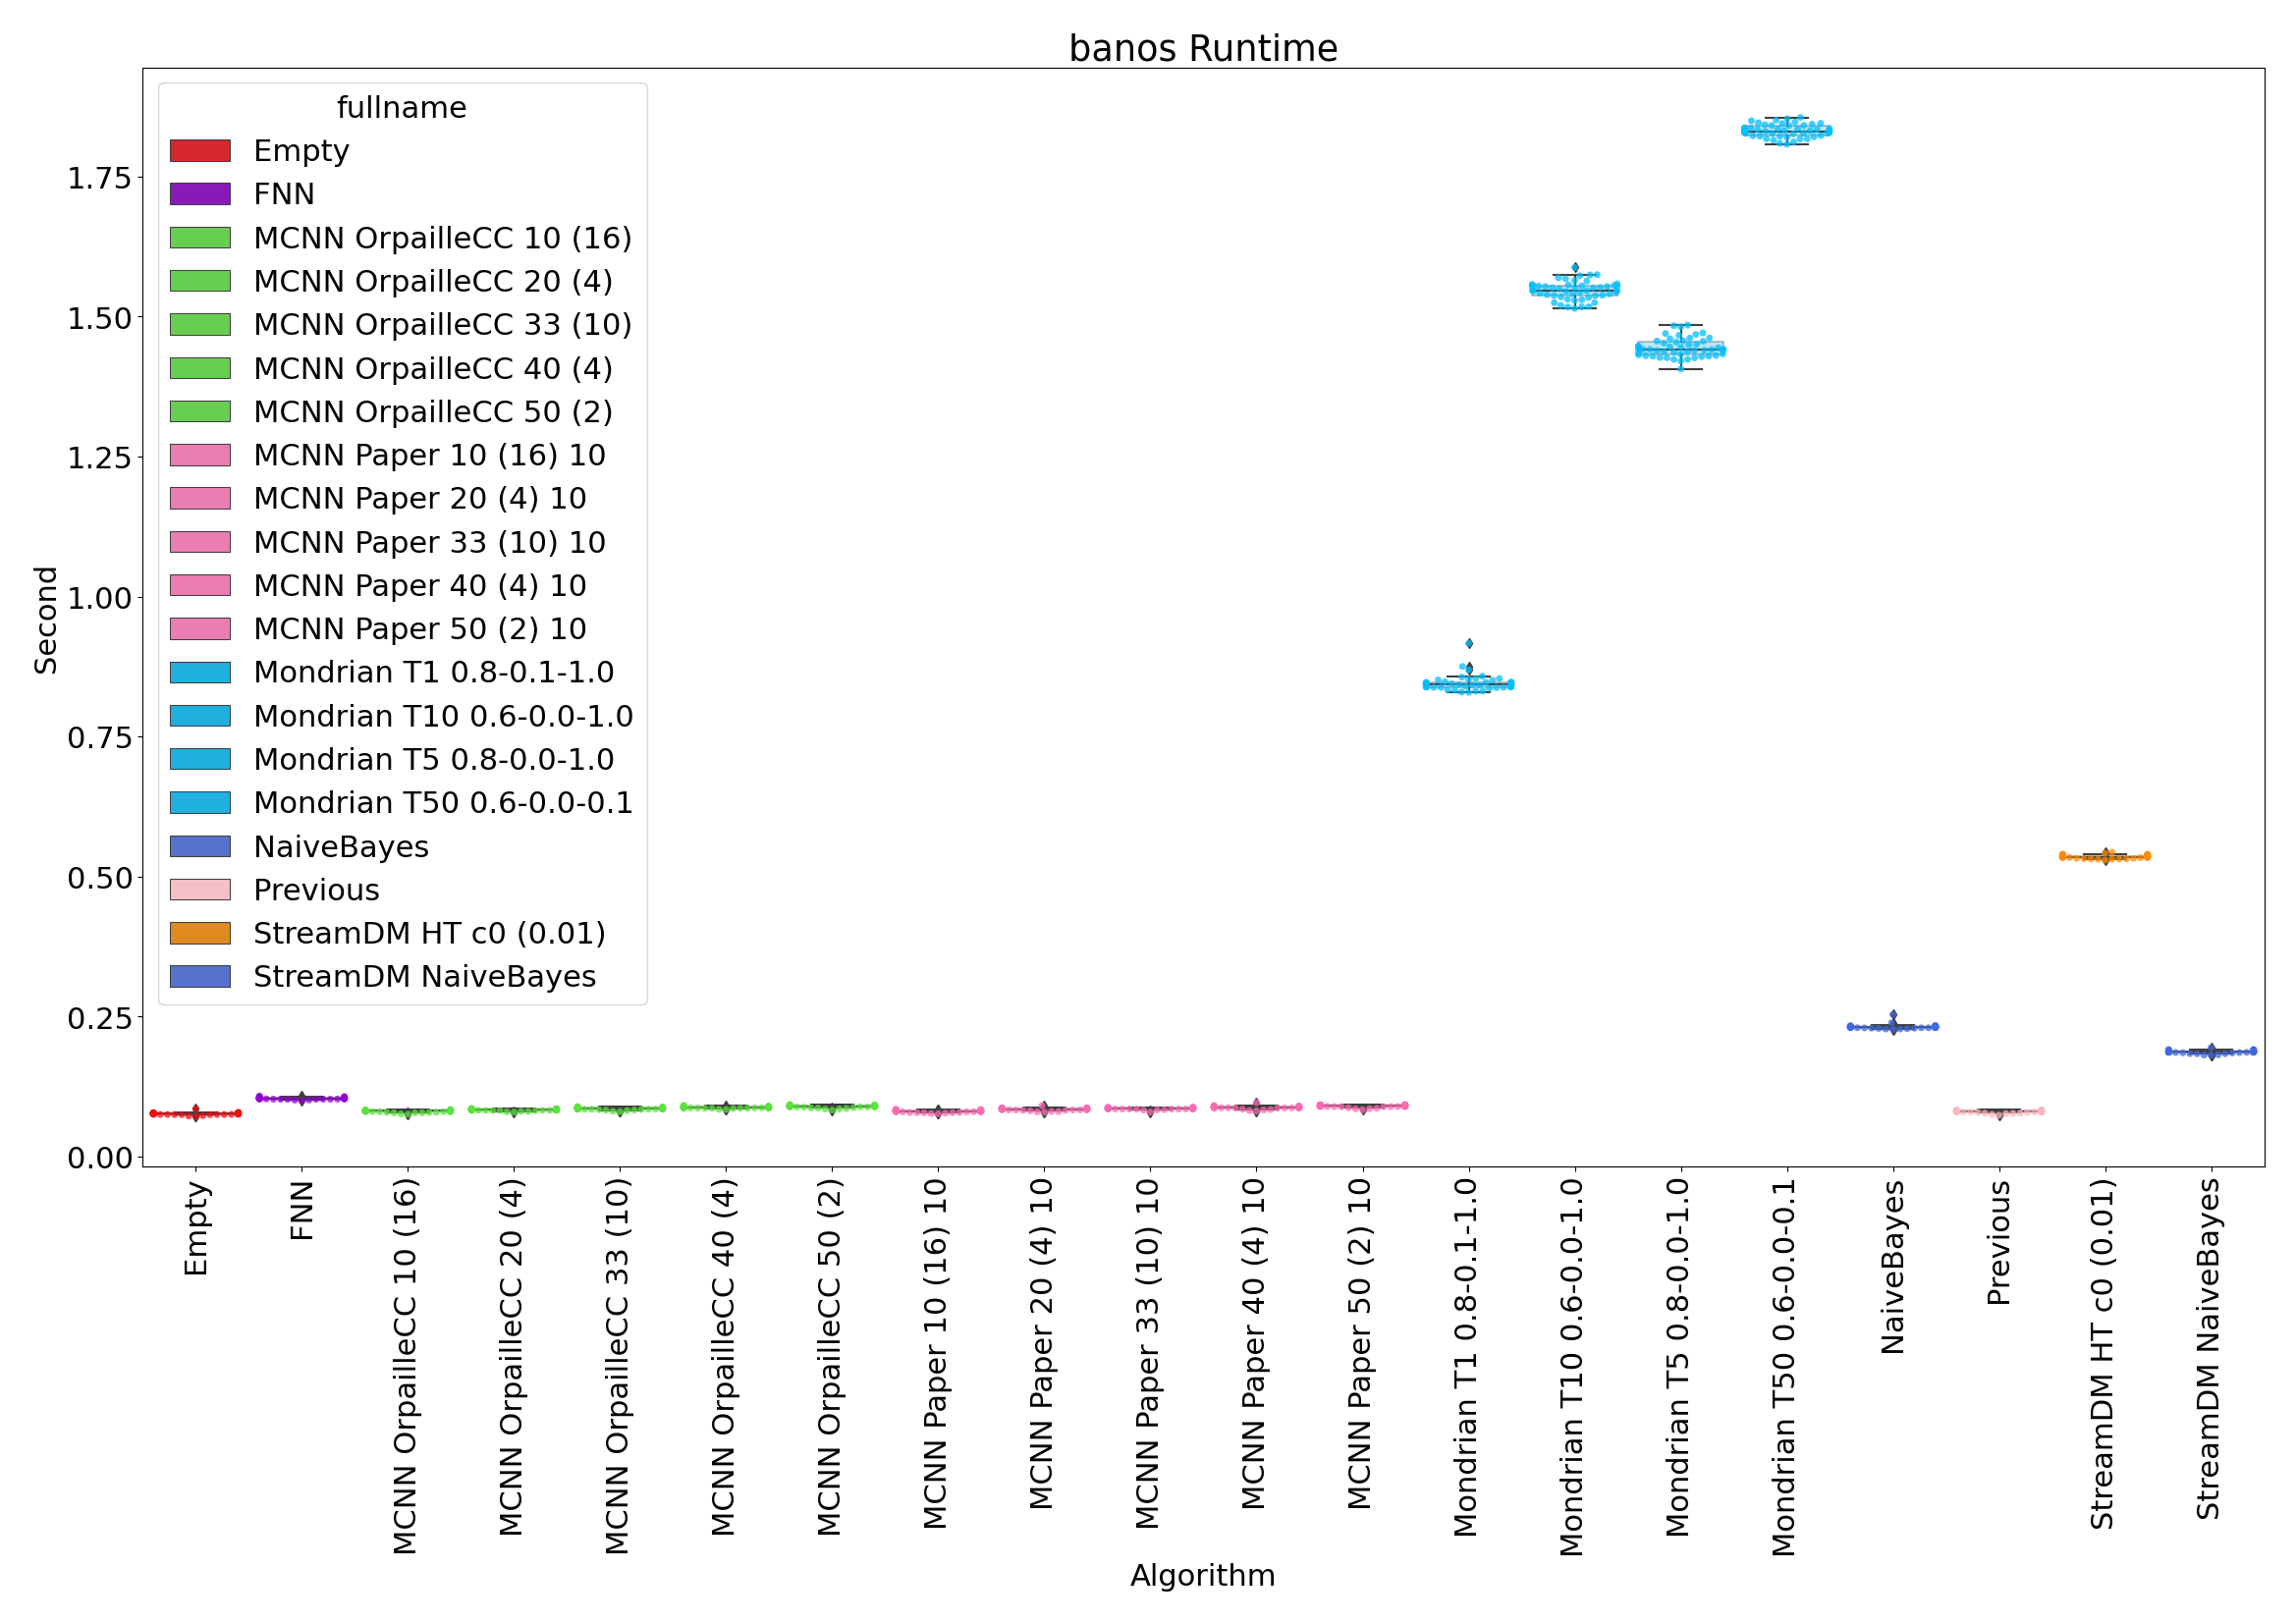
\includegraphics[width=\linewidth]{figures/results/banos_runtime.png}
	\caption{Runtime on the Banos dataset.}
\end{figure}
\begin{figure}[H]
	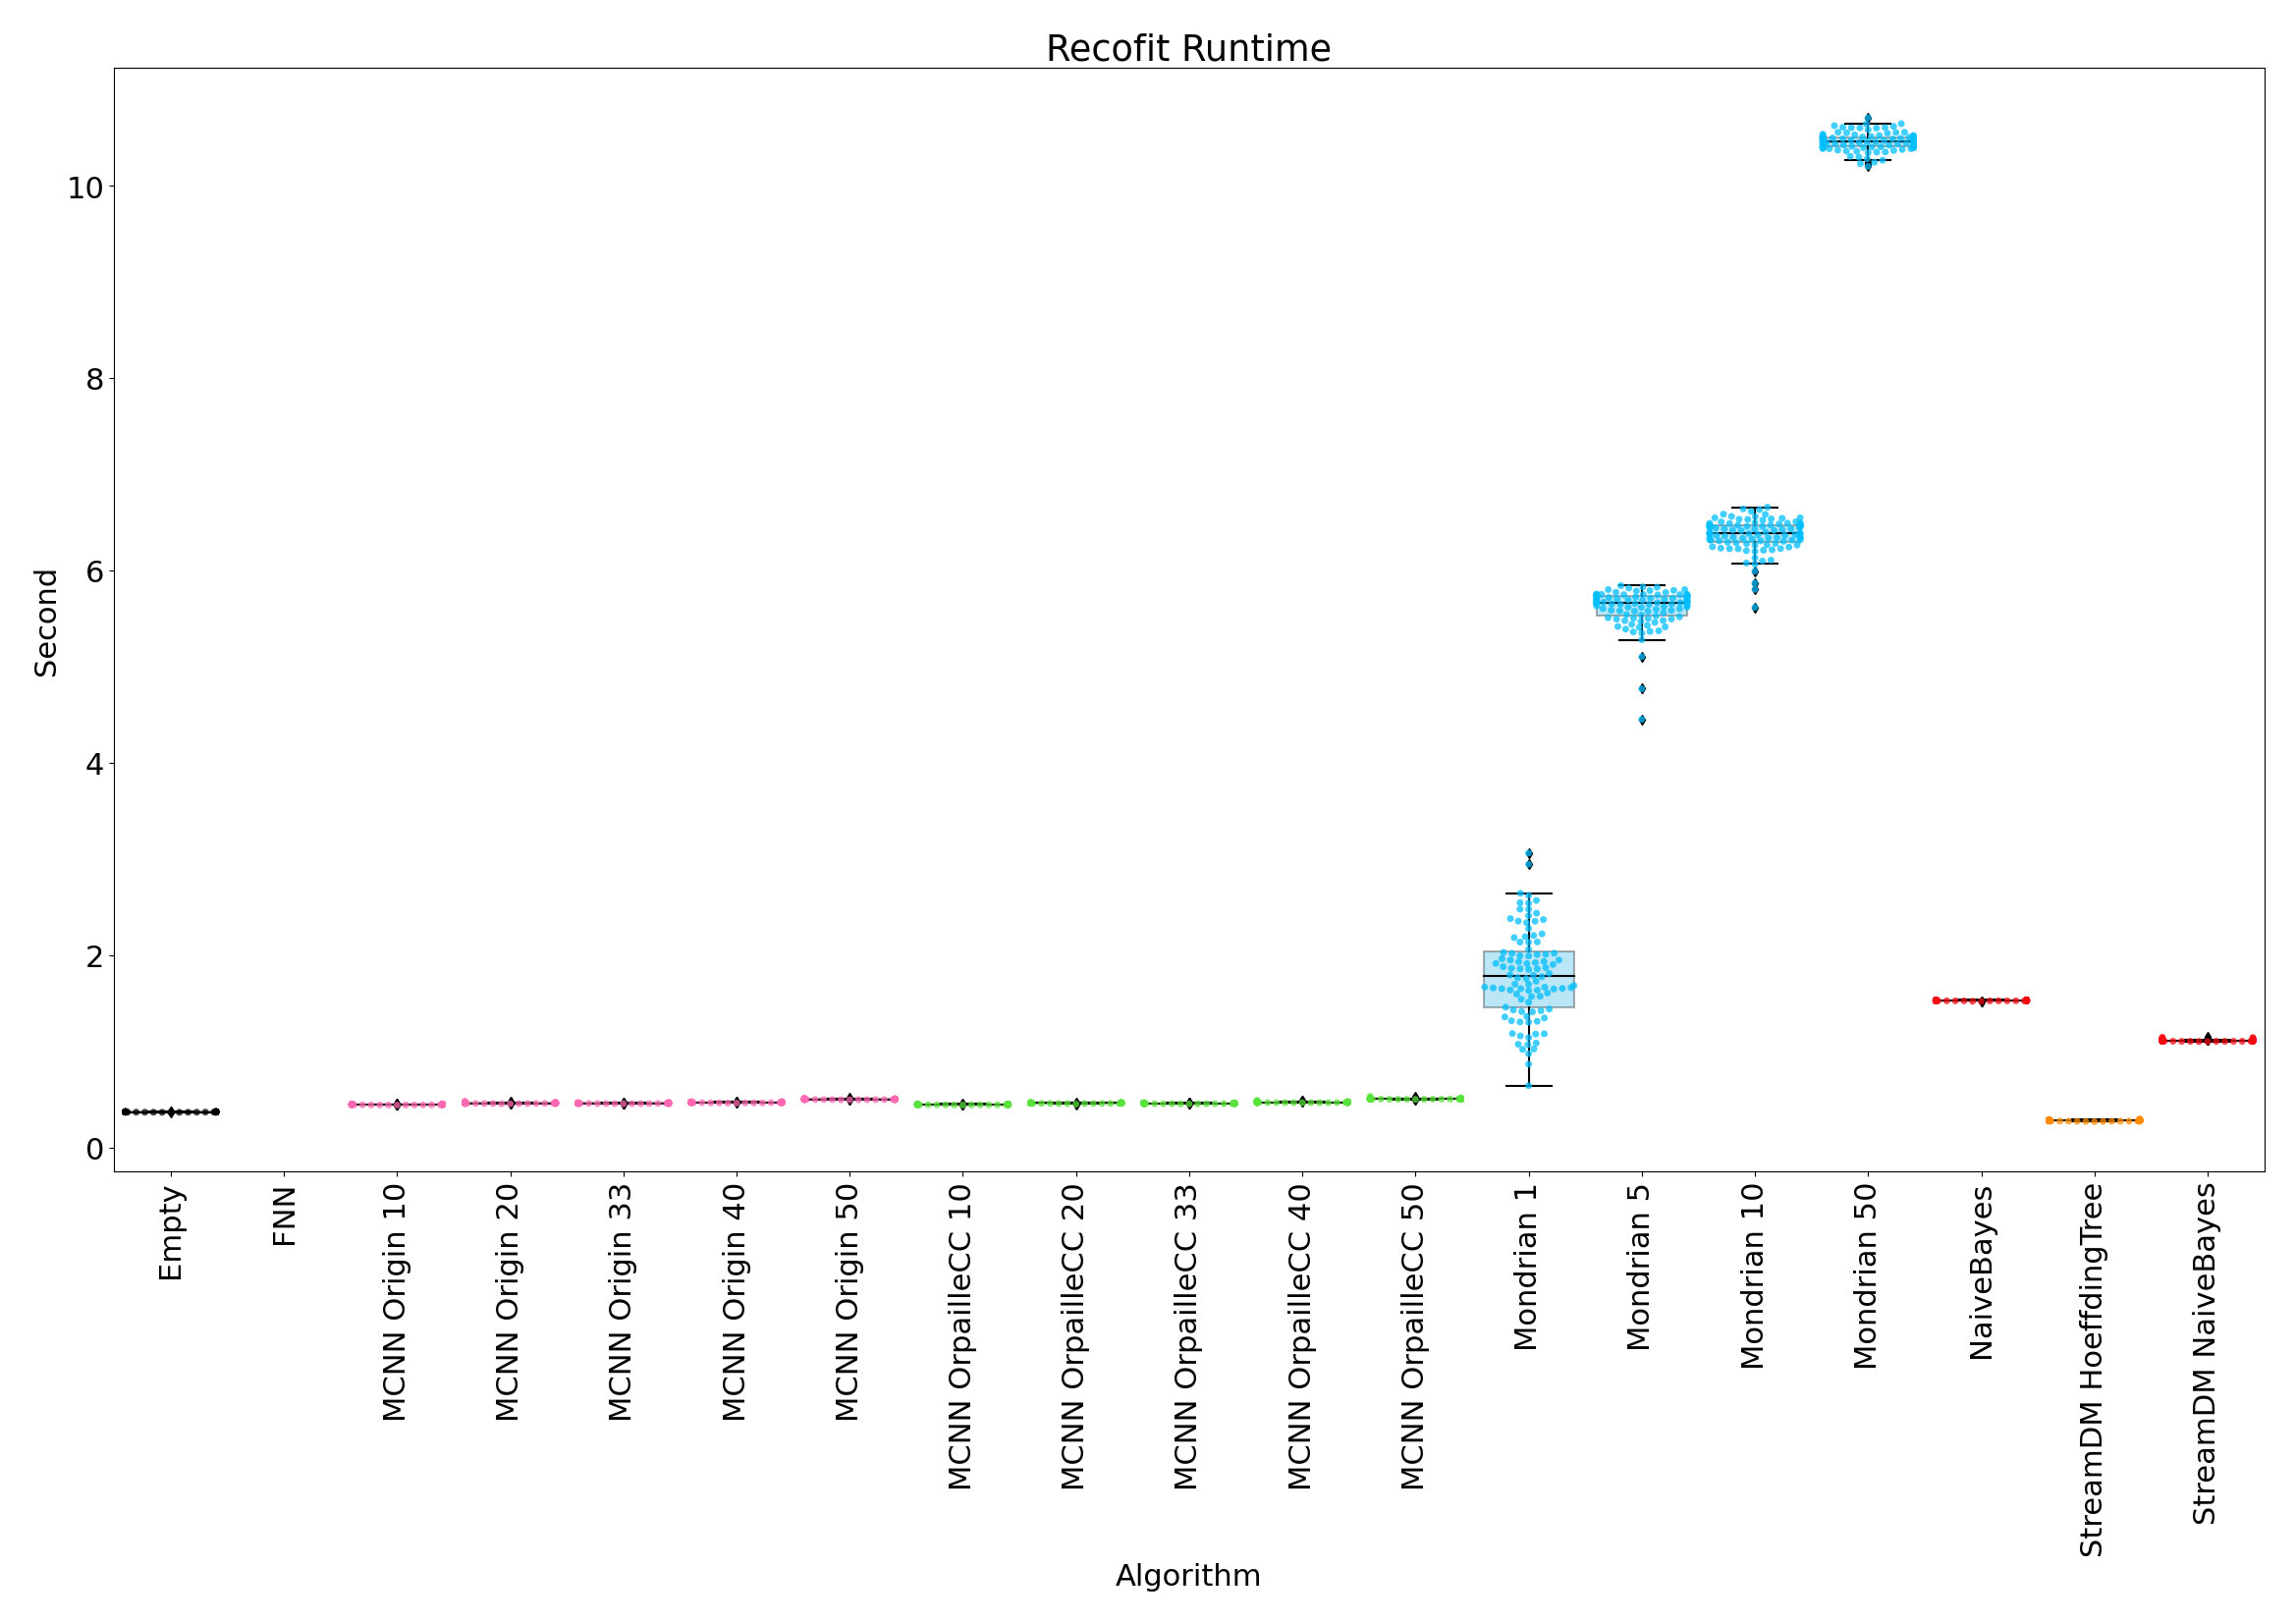
\includegraphics[width=\linewidth]{figures/results/recofit_runtime.png}
	\caption{Runtime on the Recofit dataset.}
\end{figure}

\subsection{Memory}
\begin{figure}[H]
	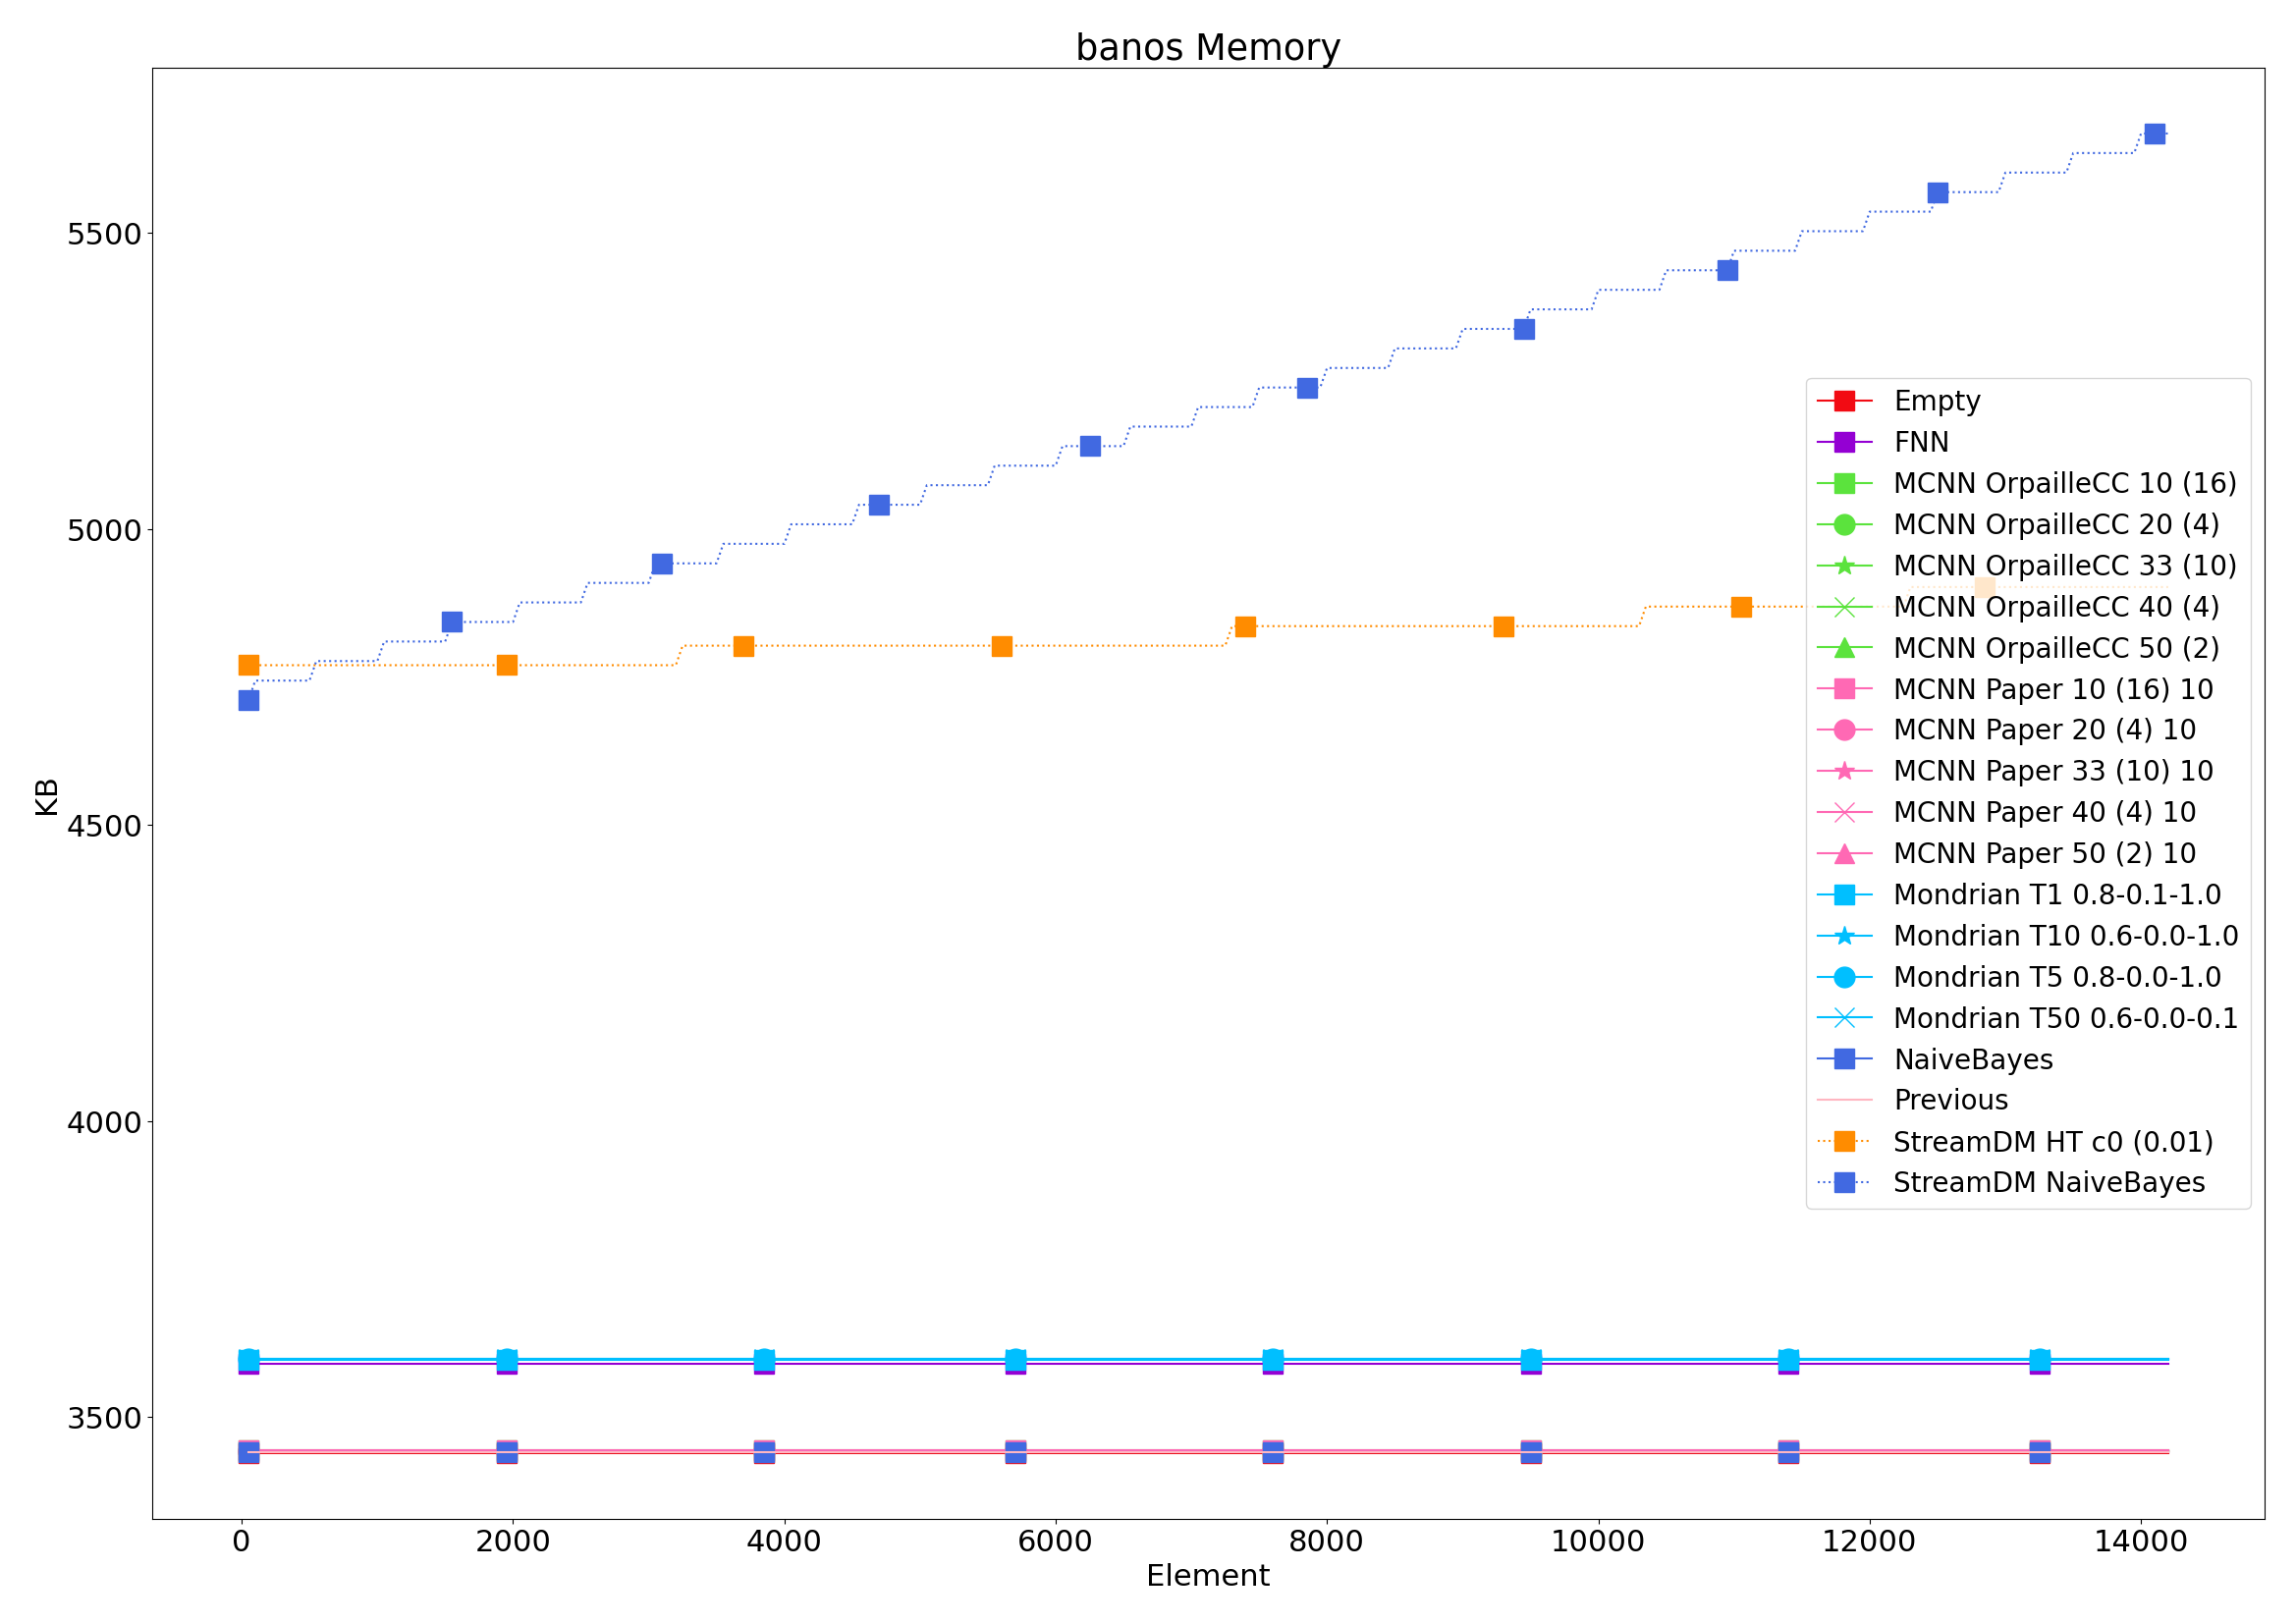
\includegraphics[width=\linewidth]{figures/results/banos_memory.png}
	\caption{Memory used by the algorithms on the Banos dataset.}
\end{figure}


\subsection{Micro-Cluster Nearest Neighbor tuning}
Figure~\ref{fig:mcnn-tuning-error} show the impact of the error threshold on different number of cluster.
\begin{figure}[H]
     \begin{subfigure}[b]{0.49\textwidth}
         \centering
		 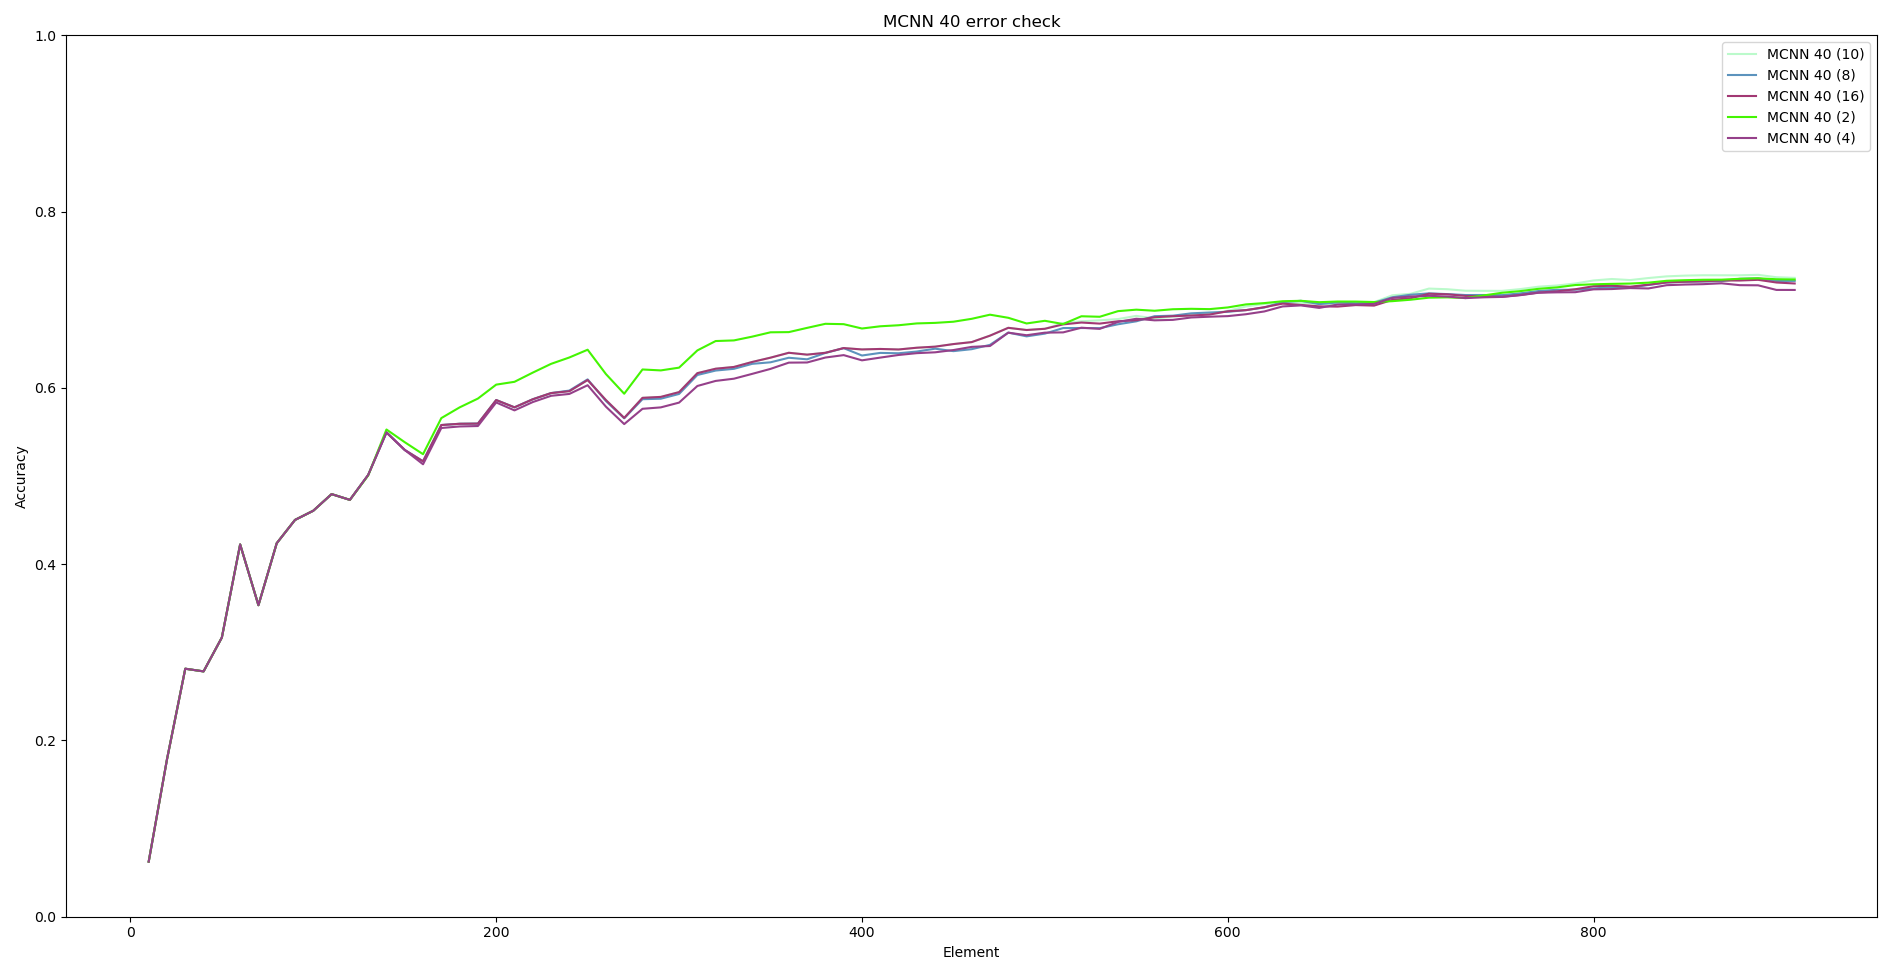
\includegraphics[width=\linewidth]{figures/Banos_S1_shuf_MCNN_40_error_check.png}
         \caption{40 clusters}
     \end{subfigure}
     \begin{subfigure}[b]{0.49\textwidth}
         \centering
		 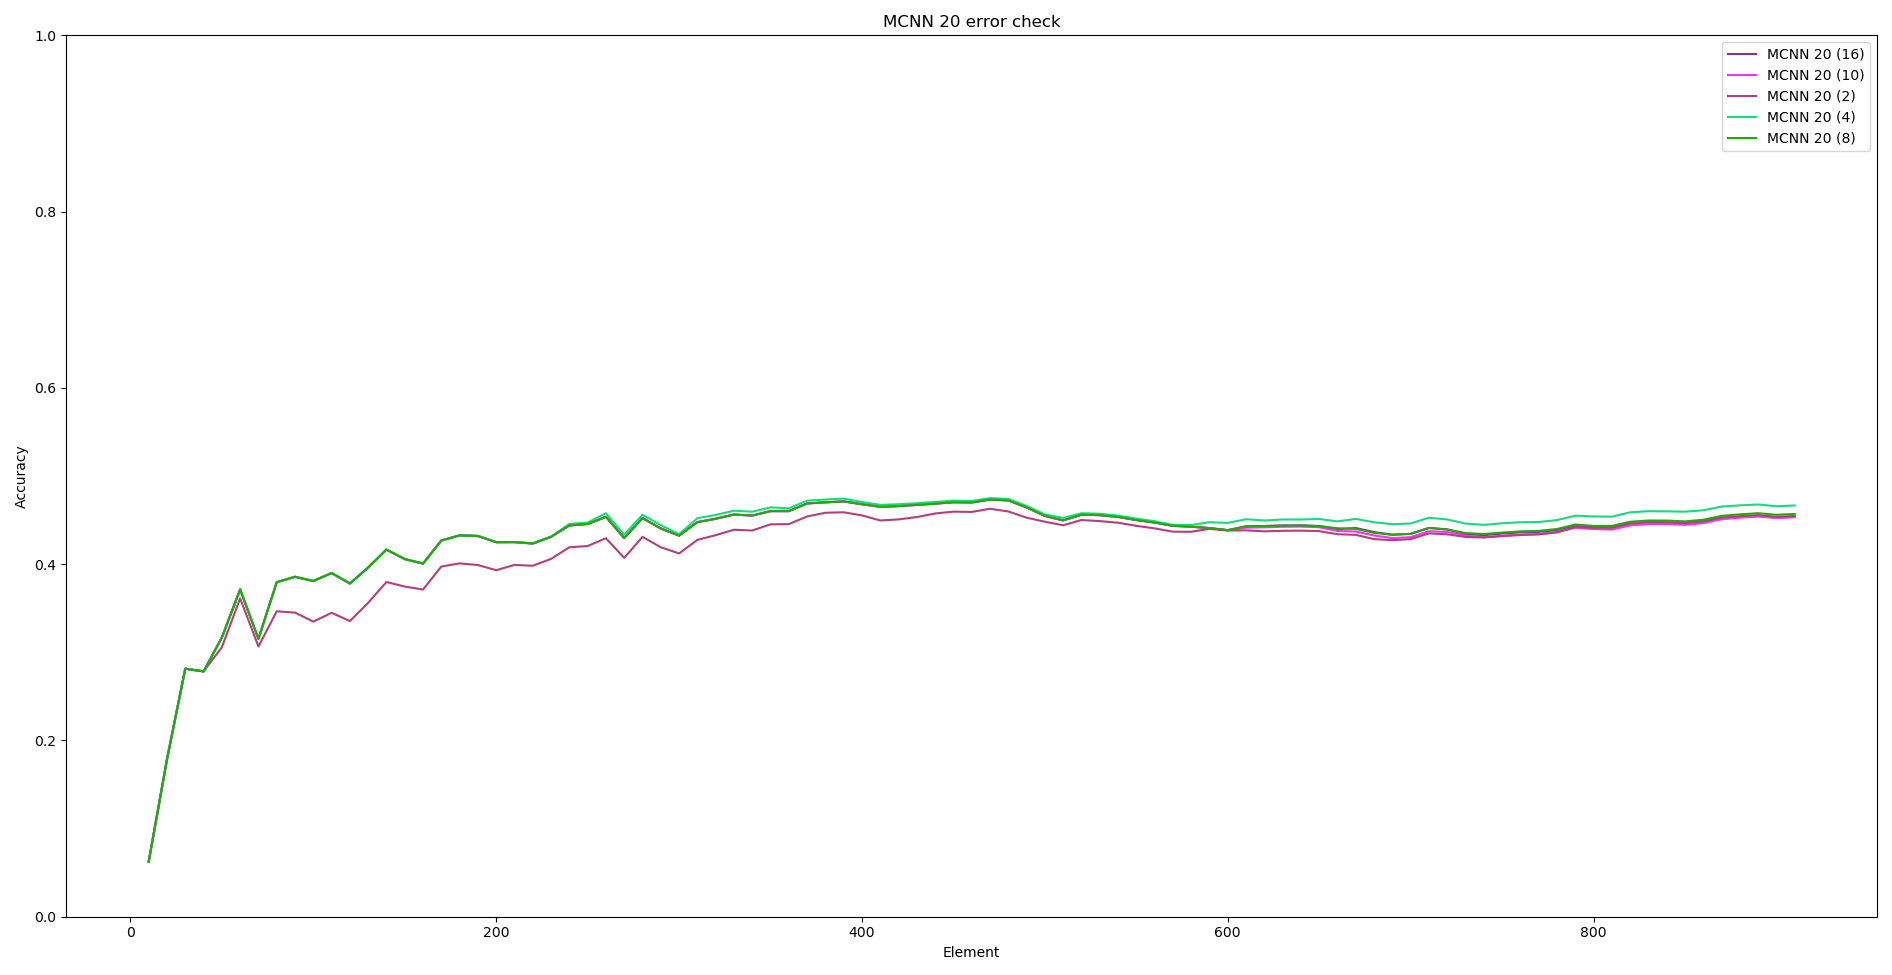
\includegraphics[width=\linewidth]{figures/Banos_S1_shuf_MCNN_20_error_check.png}
         \caption{20 clusters}
     \end{subfigure}
     \begin{subfigure}[b]{0.49\textwidth}
         \centering
		 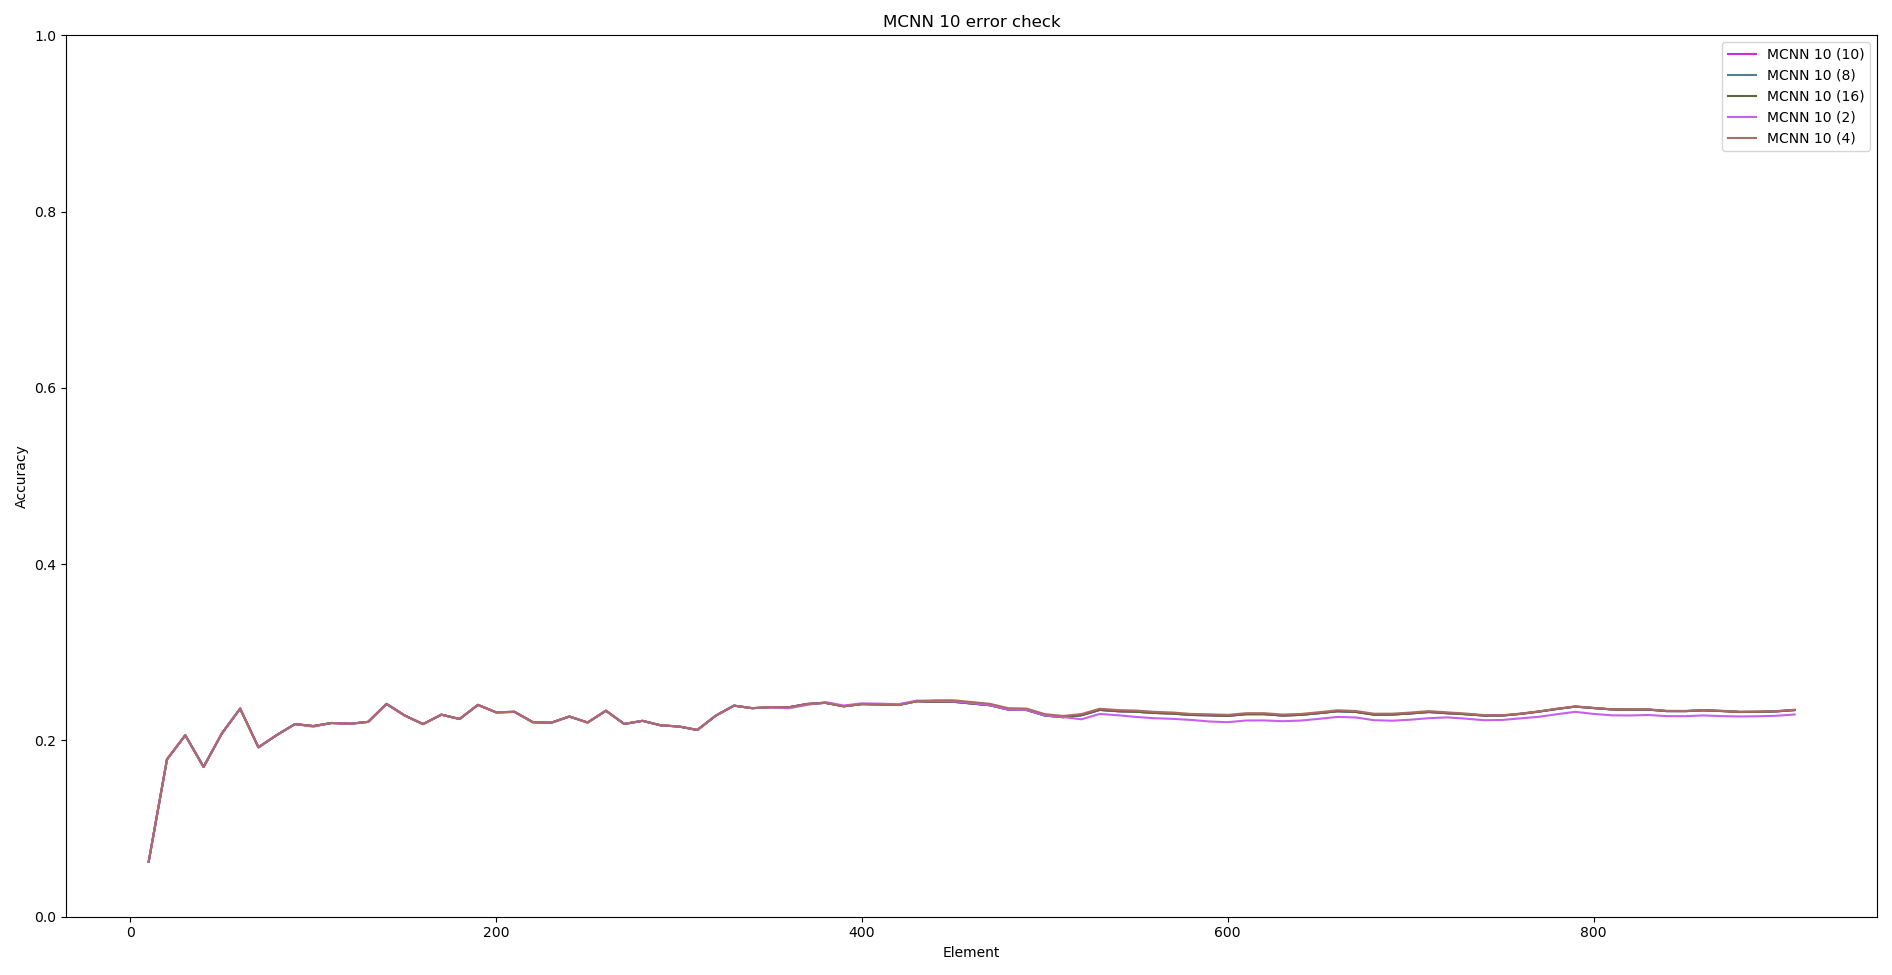
\includegraphics[width=\linewidth]{figures/Banos_S1_shuf_MCNN_10_error_check.png}
         \caption{10 clusters}
     \end{subfigure}
	\caption{MCNN error}
	\label{fig:mcnn-tuning-error}
\end{figure}

\subsection{Mondrian Tuning}
Figure~\ref{fig:mondrian-tuning} show the impact of the Mondrian parameters on
the accuracy. Occasionnaly, dashed lines are used to emphasis the minimum and
the maximum.
\begin{figure}
     \centering
     \begin{subfigure}[b]{0.49\textwidth}
         \centering
         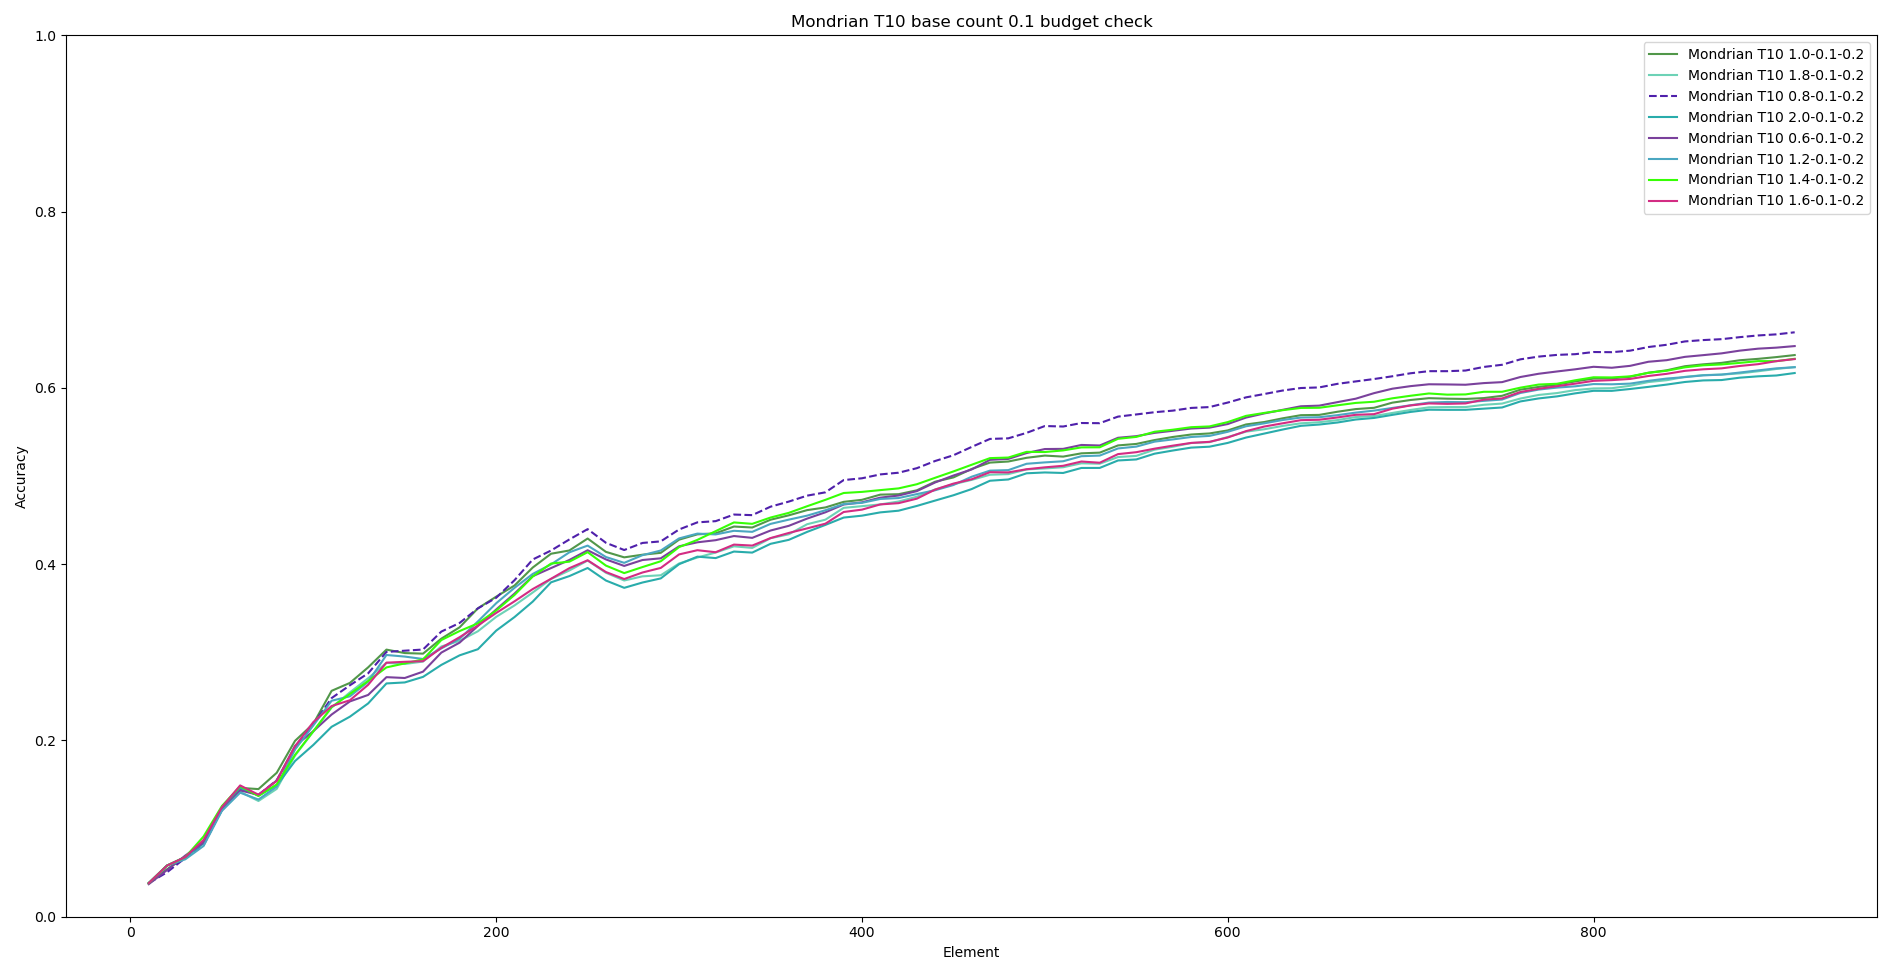
\includegraphics[width=\textwidth]{figures/Banos_S1_shuf_Mondrian_T10_bc_0.1_budget_check.png}
         \caption{Impact of the $budget$ with 10 trees, a base count of $0.1$, and discount factor of $0.2$.}
     \end{subfigure}
     \hfill
     \begin{subfigure}[b]{0.49\textwidth}
         \centering
         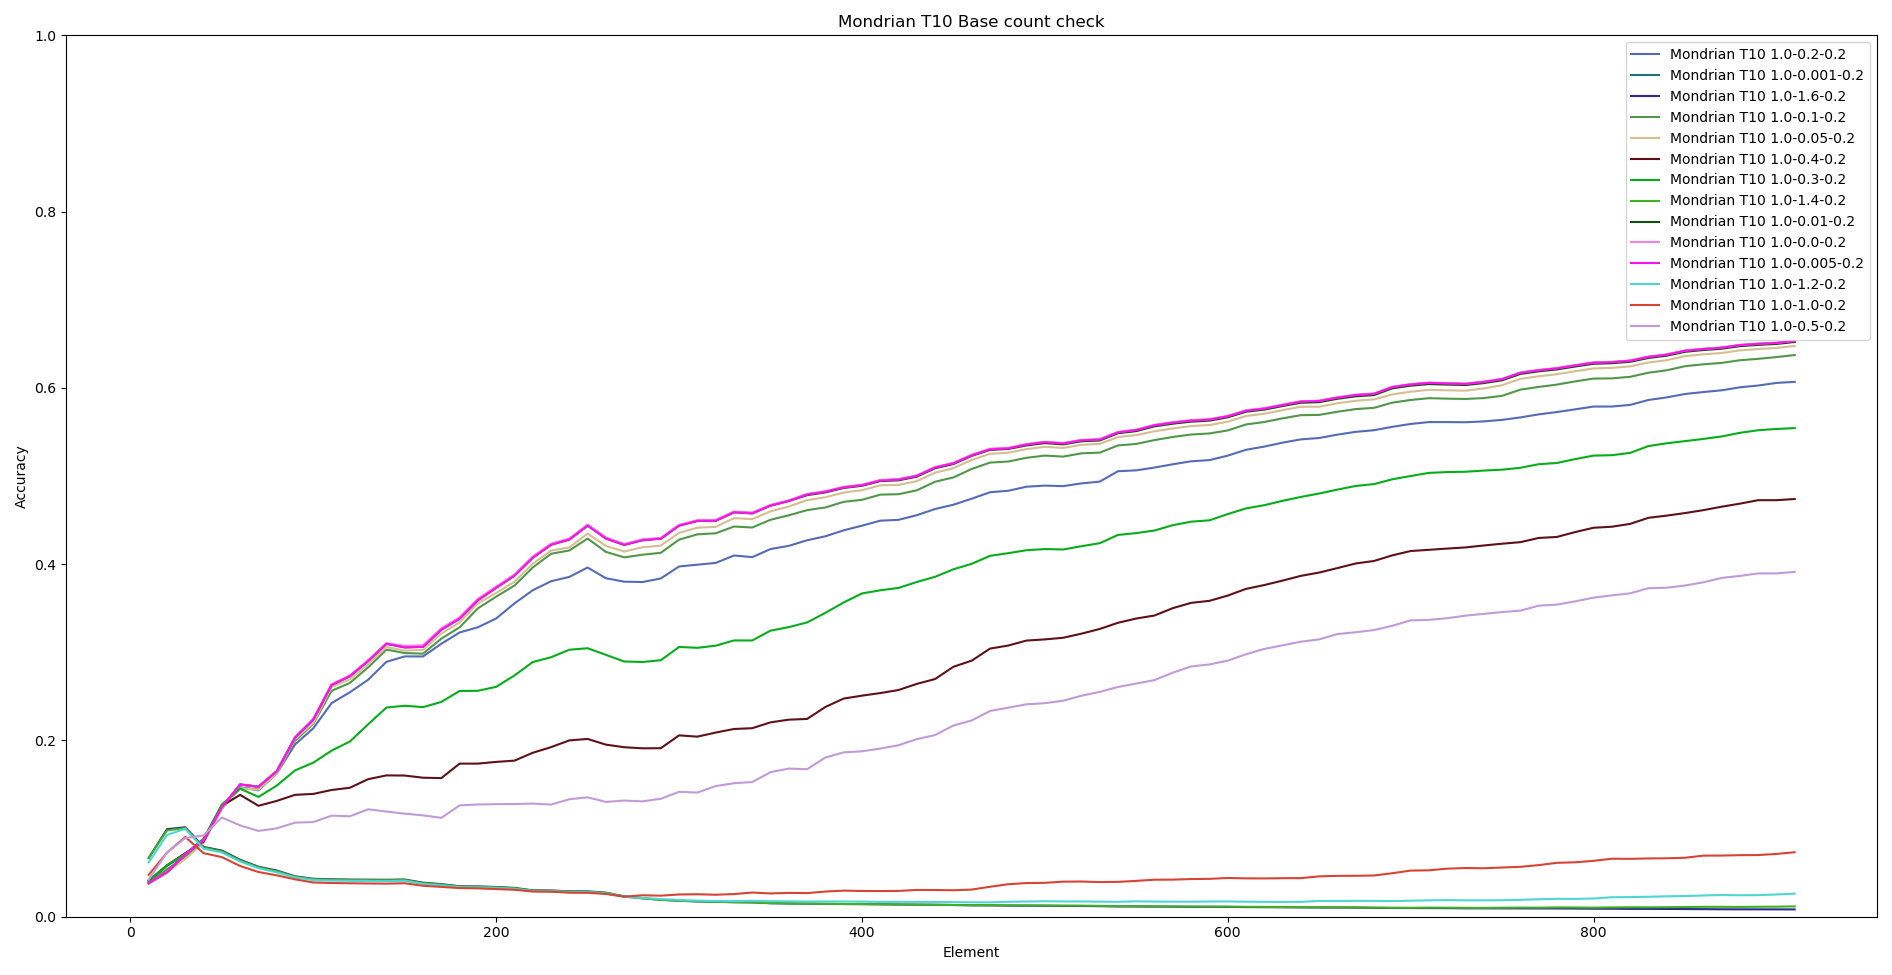
\includegraphics[width=\textwidth]{figures/Banos_S1_shuf_Mondrian_T10_check.png}
         \caption{Impact of the base count with 10 trees, a budget of $1.0$, and a discount factor of $0.2$.}
     \end{subfigure}
     \hfill
     \begin{subfigure}[b]{0.49\textwidth}
         \centering
         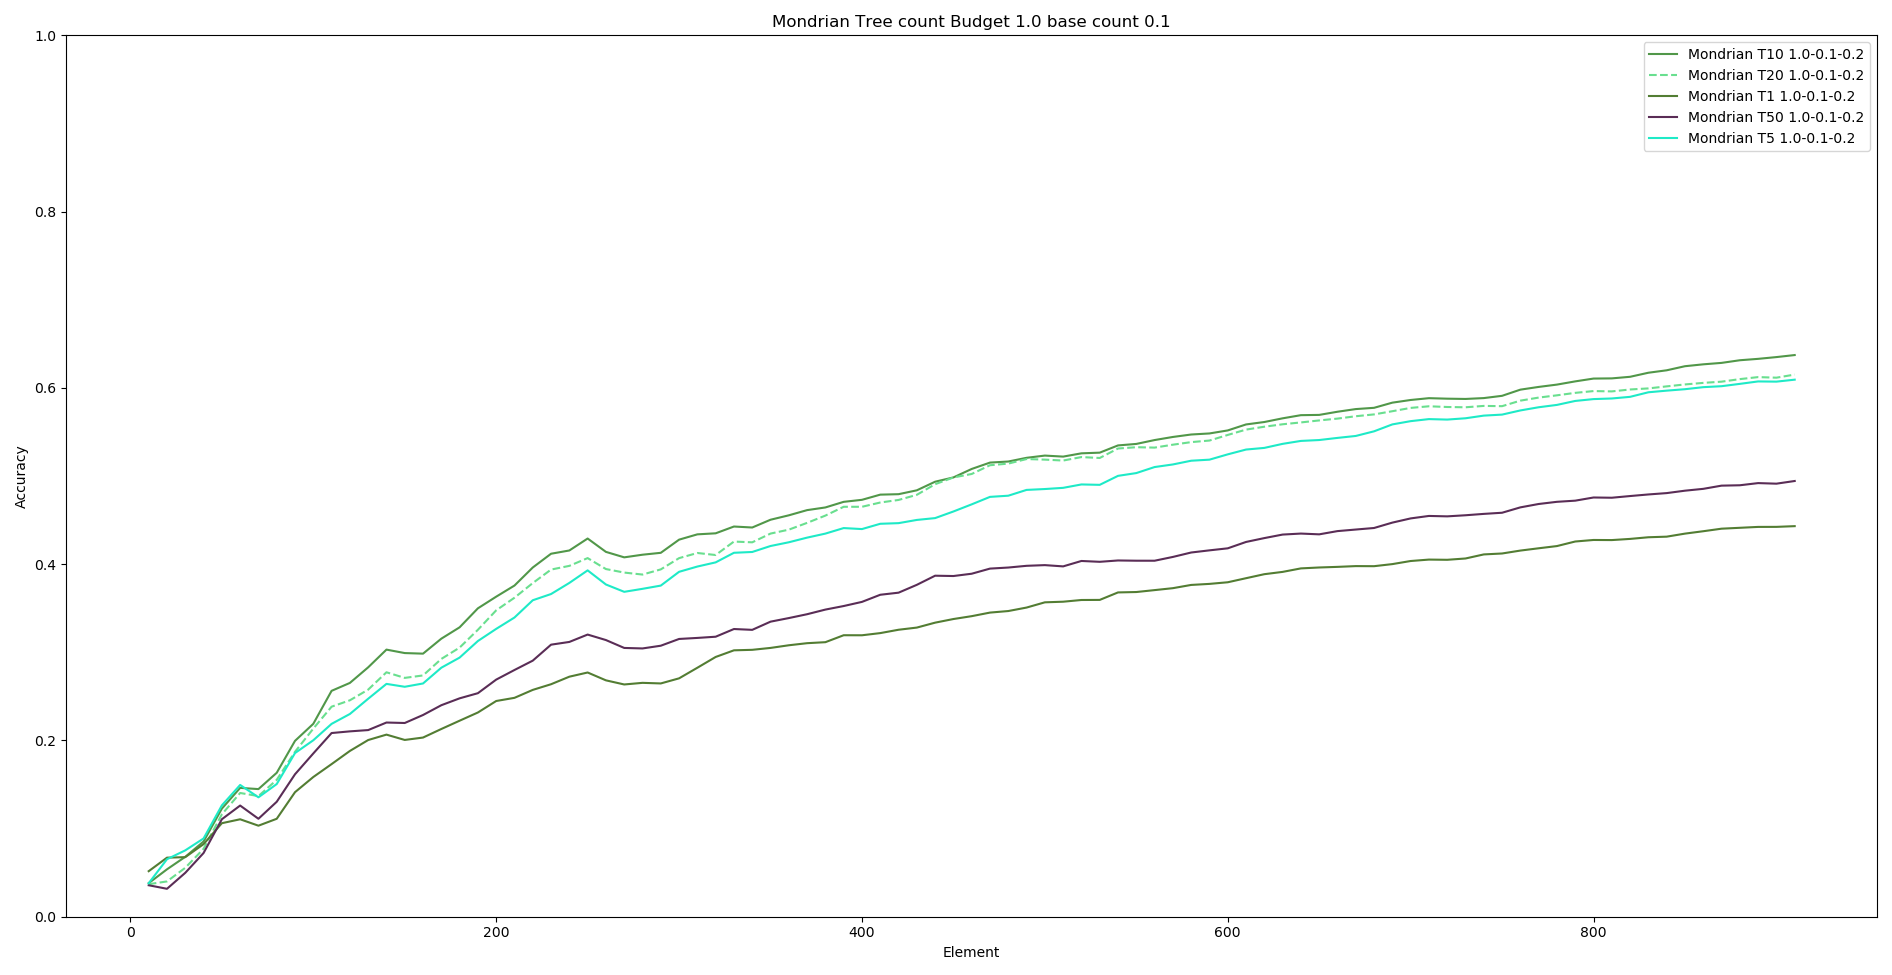
\includegraphics[width=\textwidth]{figures/Banos_S1_shuf_Mondrian_tree_count_fixed_other_bc0.1.png}
         \caption{Impact of the tree count with a budget of $1.0$, a base count of $0.1$, and a discount factor of $0.2$.}
     \end{subfigure}
     \begin{subfigure}[b]{0.49\textwidth}
         \centering
         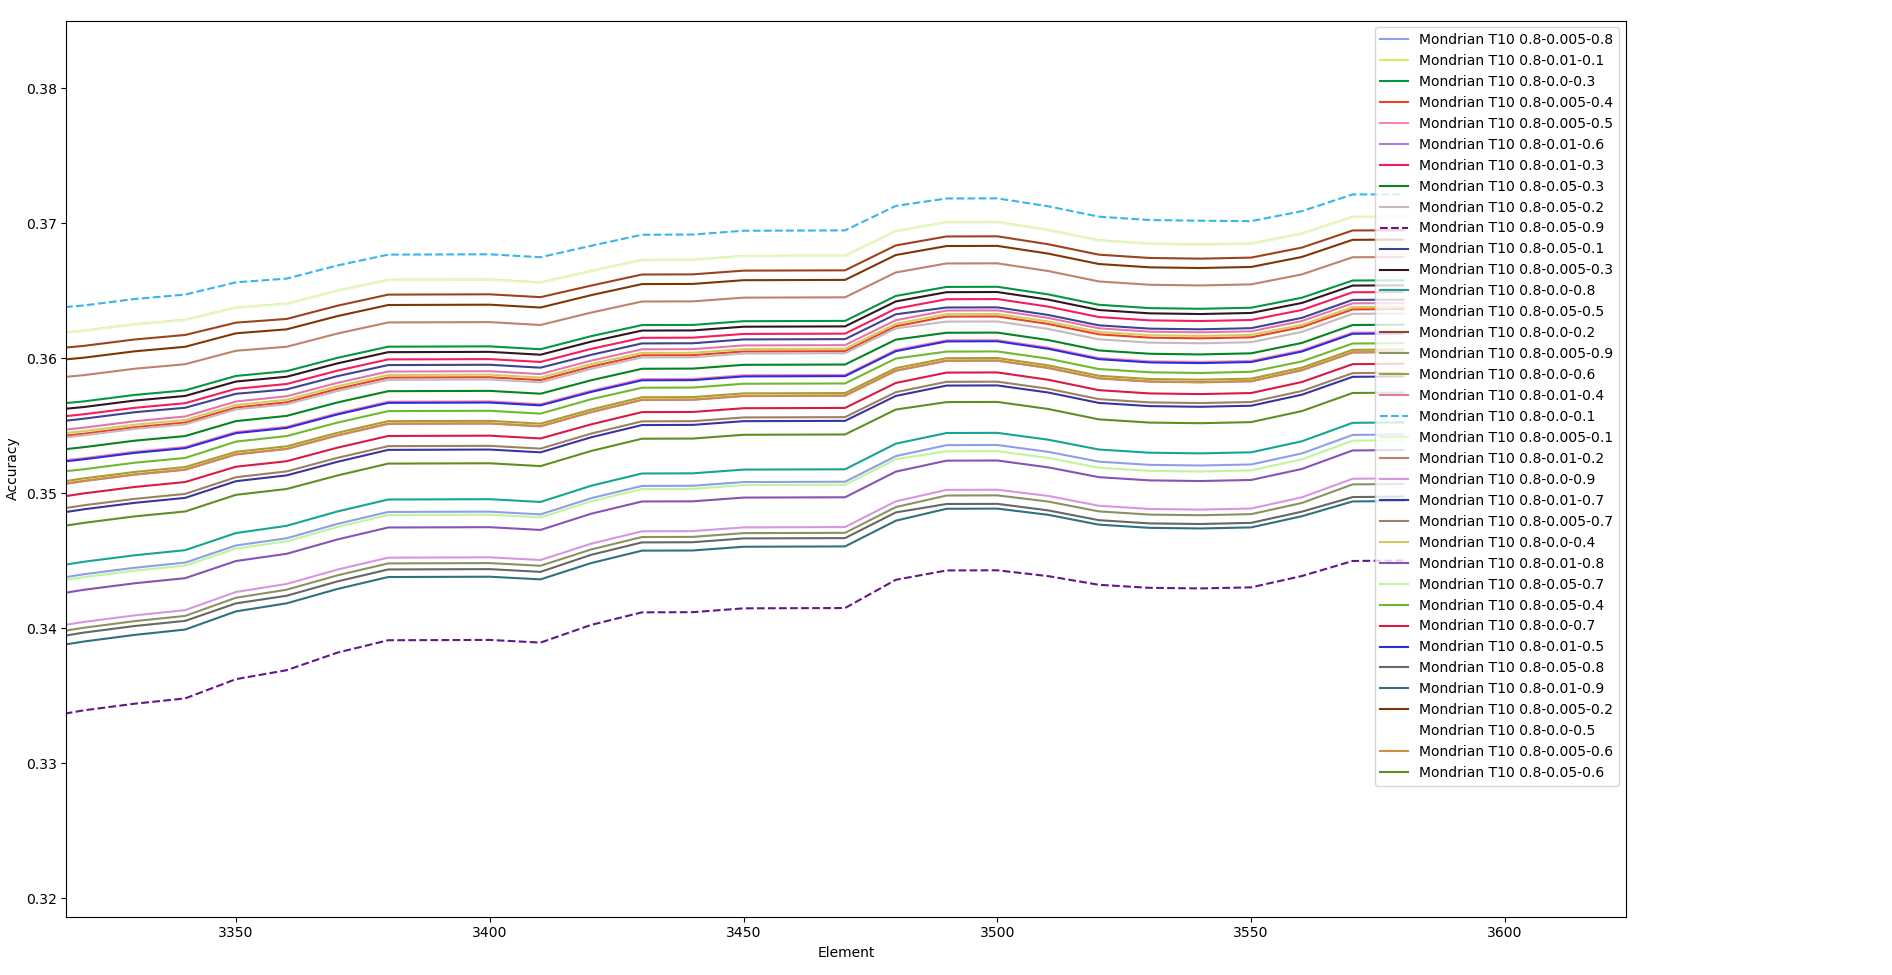
\includegraphics[width=\textwidth]{figures/Banos_S1_disount_check.png}
         \caption{Impact of the discount factor with 10 trees, a budget of $1.0$, and a base count of $0.1$.}
     \end{subfigure}
        \caption{Mondrian tuning results.}
        \label{fig:mondrian-tuning}
\end{figure}

